%-------------------------------------------------------------------------------
% paper/cace/main.tex -- "Choupo: an open-source chemical process simulator
% for education and research", the full research article drafted for
% Computers & Chemical Engineering (Elsevier) (DEV.md 4c C126).
%
% REVISION 2 (2026-10-25), from the external review kept at
% reviews/2026-10-21-external-review.md (major revision).  The point-by-point
% answer is reviews/2026-10-25-response-to-reviewers.md.  The supplement is
% supplement.tex (built by the Makefile beside this file).
%
% Prose: CC BY-SA 4.0 in the repository (the licence the journal's publishing
% agreement takes at acceptance is a decision for the authors -- TODO A9).
% Code excerpts and case files quoted in it: GPL-3.0-or-later.
%
% Build (from this directory):  make        -- see the Makefile header.
%
% EVIDENCE RULE (C126): every factual claim about the engine carries, in a
% LaTeX comment beside it, the file, the check or the run it was READ at.
% EVERY ENGINE NUMBER IN THIS REVISION WAS RE-READ FROM A RUN on the tree of
% branch claude/c126-papers-revision (origin/main c11d0354a, 2026-10-25, plus
% the benchmark-case changes this revision makes, listed in the response to
% reviewers): `make all -j3`, each case copied to a scratch directory and run
% with the binary its controlDict names; the benchmarks with
% `python3 -I benchmarks/dwsim/compare.py <case>`.  The commands are in
% supplement.tex, section S1.  Counts are read from generated files at
% 3e5d03c52 (generated/releaseInventory.json, generated/gateManifest.json) and
% e63941d79 (generated/methodTools.json), never typed from memory.
%
% THE JOURNAL'S GUIDE FOR AUTHORS COULD NOT BE READ (HTTP 403 on 2026-10-21).
% Everything below follows general Elsevier conventions; each is an
% ASSUMPTION for the authors to check (TODO A1-A9, unchanged from revision 1):
%   A1 article type (research article, ~30 pp preprint; no length limit read);
%   A2 highlights 3-5 x <= 85 characters (make check-highlights);
%   A3 abstract <= 250 words, 1-7 keywords;  A4 graphical abstract file;
%   A5 numbered references (elsarticle-num-names);  A6 the exact wording and
%   place of the generative-AI declaration;  A7 line numbers / spacing;
%   A8 data/code availability section and software DOI;  A9 article licence.
%
% TODO (authors) -- Vitor's decisions, owed:
%   B1 affiliations, ORCIDs, e-mails, corresponding author (placeholders);
%   B2 CRediT roles of Pedro Mendes and Miguel Rodrigues;
%   B3 competing interests and the trade-mark disclosure;
%   B4 THE VERSION THIS ARTICLE CITES.  The reviewer asks for one frozen,
%      fully re-run version.  This revision re-ran every number on one
%      commit of the development line (named in the Data availability
%      section); a release TAG (vYYMM) cut from that commit, and a Zenodo
%      archive of it, are Vitor's to decide (B6);
%   B5 Section 5.4 goes public only after the reference's findings have been
%      offered upstream (paper/whitepaper/upstream-issue-draft.md covers case
%      B only);  B6 Zenodo DOI;  B7 funding;
%   B8 references -- every entry was re-checked against Crossref on
%      2026-10-25 where the item has a DOI; the ones that could not be checked
%      carry a TODO in refs.bib (cavett1963, choi1986, nasa7009, wang1966,
%      cantera's Zenodo DOI, dwsim);
%   B9 classroom evaluation (none exists; stated in Sections 1 and 7);
%   B10 the two curation datasets of Section 4 have NOT been read back against
%      their articles (the reviewer asks for it; it is a curator's act);
%   B11 the CACHE News article of 2005 that publishes a second Cavett solution
%      is not cited: its title names a commercial simulator, and the
%      project's naming rule (CLAUDE.md sec 10) forbids naming one.  Cite it
%      in full (which needs that rule's exception for one reference) or keep
%      it out, as this revision does.
%
% THE DRAFT SWITCH: \drafttrue prints a DRAFT watermark and numbers the lines.
%-------------------------------------------------------------------------------
\newif\ifdraft
\drafttrue

\documentclass[preprint,12pt]{elsarticle}

\usepackage[T1]{fontenc}
\usepackage[utf8]{inputenc}
\usepackage{lmodern}
\usepackage[english]{babel}
\usepackage{amsmath}
\usepackage[a4paper,margin=2.5cm,footskip=1.1cm]{geometry}
\usepackage{microtype}
\usepackage{booktabs}
\usepackage{tabularx}
\usepackage{array}
\usepackage{xcolor}
\usepackage{listings}
\usepackage{graphicx}
% Figures: figures/ holds the TikZ shared with the graphical abstract; the
% white paper's folder holds the curation run's data (one home).  The data
% this revision adds (nanofiltration) live in data/, each file written by a
% generator in figures/ (supplement S1).
\graphicspath{{figures/}{../whitepaper/figures/}}
\newcommand{\datadir}{../whitepaper/data}
\newcommand{\cacedata}{data}
\usepackage{tikz}
\usetikzlibrary{positioning,fit,arrows.meta,calc}
\usepackage{pgfplots}
\pgfplotsset{compat=1.17}
\usepgfplotslibrary{groupplots}
\usepackage{enumitem}
\usepackage{placeins}
\usepackage{needspace}
\setlist{itemsep=2pt,topsep=4pt}
\definecolor{linkink}{RGB}{20,60,110}
\definecolor{fitink}{RGB}{180,60,20}
\definecolor{heldink}{RGB}{20,90,160}
\definecolor{unifacink}{RGB}{40,130,70}
\definecolor{idealink}{RGB}{120,120,120}
\usepackage[colorlinks=true, linkcolor=linkink,
            citecolor=linkink, urlcolor=linkink]{hyperref}
\biboptions{sort&compress}

\ifdraft
  \usepackage{draftwatermark}
  \DraftwatermarkOptions{text=DRAFT, angle=45, fontsize=3cm,
                         color={gray!18}}
  \usepackage{lineno}
\fi

\newcommand{\code}[1]{\texttt{\detokenize{#1}}}
\makeatletter
\g@addto@macro\UrlBreaks{\do\-\do\_}
\makeatother
\newcommand{\brk}[1]{\nolinkurl{#1}}
\newcommand{\OF}{OpenFOAM}

\lstset{basicstyle=\ttfamily\scriptsize, columns=fullflexible,
        keepspaces=true, frame=single, rulecolor=\color{gray!50},
        xleftmargin=4pt, xrightmargin=4pt, aboveskip=6pt, belowskip=6pt,
        upquote=true,
        literate={γ}{{$\gamma$}}1 {φ}{{$\varphi$}}1 {Δ}{{$\Delta$}}1
                 {→}{{$\rightarrow$}}2 {·}{{$\cdot$}}1}

\journal{Computers \& Chemical Engineering}

\begin{document}

\begin{frontmatter}

\title{Choupo: an open-source chemical process simulator for education and
research}

% TODO B1: affiliations, ORCIDs, e-mails, corresponding author.
\author[inst1]{Vítor Geraldes\corref{cor1}}
\ead{TODO (authors)}
\author[inst1]{Pedro Mendes}
\author[inst1]{Miguel Rodrigues}
\cortext[cor1]{Corresponding author (TODO: confirm).}
\affiliation[inst1]{organization={TODO (authors): affiliation},
            city={TODO},
            country={TODO}}

\begin{abstract}
Choupo is an open-source (GPL-3.0-or-later) sequential-modular process
simulator written in C++17, for teaching and for membrane and electrolyte
research.  Its design goal is that six things are observable in
plain-text files and the run log: the data a calculation used and their
sources, its hypotheses, its equations, whether its parameters lie inside
their evidence, its iterations, and its results with conservation
balances.  We argue that the contribution is not any one of these
features, several of which exist in other open tools, but their
enforcement where every input is read and their verification across a
corpus of 494 cases.  We describe the architecture, a curation rule that
accepts a regressed parameter set only if it reproduces an independent
study within a band declared before the fit, and why that band is
conservative; and a verification method that separates numerical
convergence, physical consistency and acceptance.  The Cavett recycle
problem converges in seven Newton steps and closes its first law to
0.002~kW of 396~MW exchanged, after a mixer defect the balance report had
exposed was fixed.  Nanofiltration is treated with its equations: a
DSPM-DE pore fitted to measured chloride rejections predicts the
held-out sulfates within one rejection point but not on the transmission
scale, and a
solution-diffusion-electromigration law reproduces the published trace-ion
curves in the trace limit but not at the experiments' own concentrations.
A comparison with an open-source simulator is split into a same-equations
exercise, where a 0.6~\% conversion difference remains, and a
different-models exercise.  No classroom evaluation has been made.
\end{abstract}
% Counts: 494 = generated/releaseInventory.json tutorials.runnableCases
% (3e5d03c52).  Cavett: the run of cavett01 on this tree (Section 5.2 comment).
% Nanofiltration: membrane24 (props mode) and gen_sdem_traces.py runs.
% Benchmark E: compare.py, variant sampleKinetics (Section 5.4).

\begin{graphicalabstract}
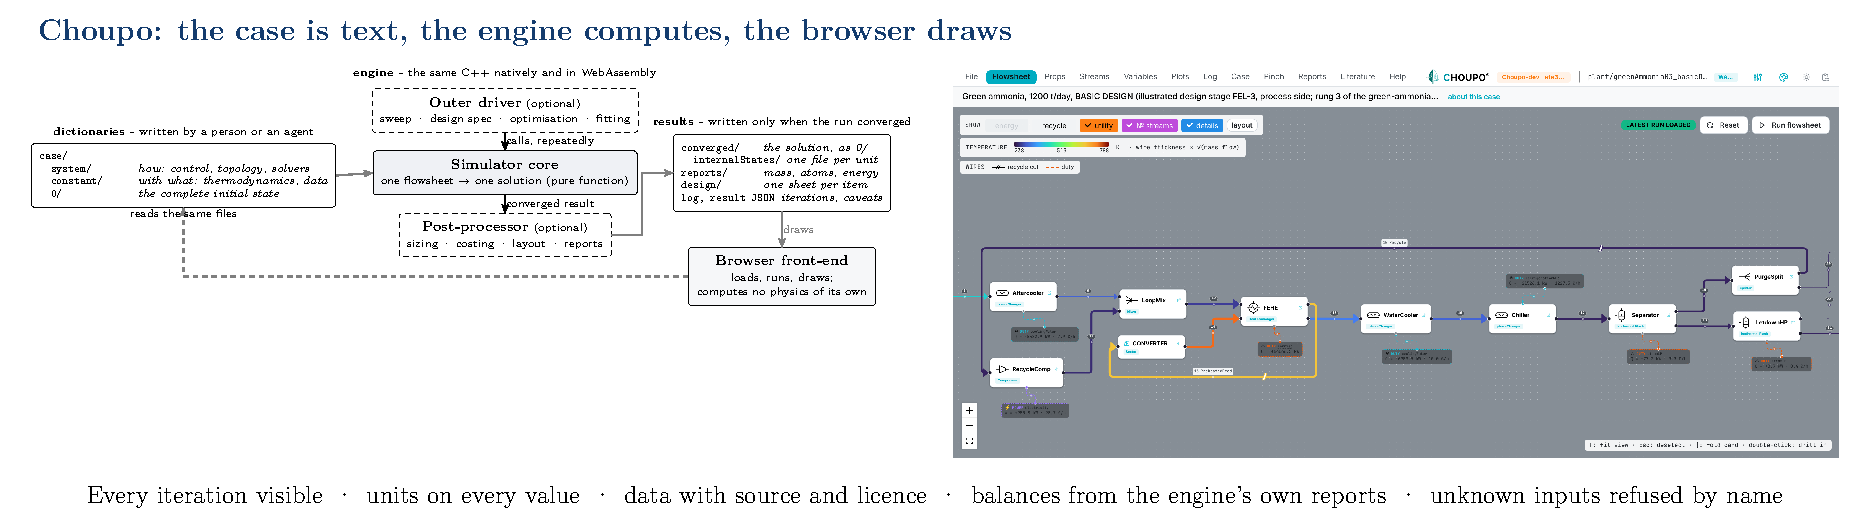
\includegraphics[width=\linewidth]{graphical_abstract.pdf}
\end{graphicalabstract}

% paper/cace/highlights.tex -- the Highlights, a separate editable file as
% Elsevier asks (TODO A2 in main.tex: 3-5 bullets, each <= 85 characters
% including spaces; the lengths are checked by `make check-highlights`).
% main.tex \inputs this file, so the bullets have one home.  Revision 2.
\begin{highlights}
\item An open process simulator that enforces six observables where inputs are read
\item Convergence, physical consistency and acceptance are reported separately
\item Regressed parameters must pass an independent study within a pre-declared band
\item A fitted nanofiltration pore holds in rejection but not in transmission
\item With identical rate laws, two simulators still differ by 0.6 \% in conversion
\end{highlights}


\begin{keyword}
process simulation \sep chemical engineering education \sep
open-source software \sep thermophysical data curation \sep
verification and validation \sep nanofiltration
\end{keyword}

\end{frontmatter}
\ifdraft\linenumbers\fi

%===============================================================================
\section{Introduction}
\label{sec:intro}

\paragraph{The problem}  A student of process simulation meets, in most
exercises, converged numbers: a column specified and solved, a recycle
that closed, stream tables to four decimals.  Whether a missing
interaction parameter was taken as zero, whether a vapour pressure was
evaluated outside the range it was fitted on, whether a recycle converged
or merely stopped, and whether the converged plant conserves energy, is
information that a simulator holds but that the exercise does not make
the student look at.  The same questions matter to a researcher who
inserts a new transport law into a plant model and must know which of
the plant's numbers the new law moved.  Choupo was written so that those
questions have answers a reader can find in files.  Whether this improves
learning is a goal, not a result: no classroom evaluation exists, and we
make no claim of one.
% CLAUDE.md sec 1 (the two audiences; "glass-box"; research areas).

\paragraph{Six observables}  We call a simulator a \emph{glass box} when a
user can observe, in plain-text files and in the run log, and without
changing a default:
\begin{enumerate}[label=(\roman*), leftmargin=2.2em]
\item the data a calculation used, and the source of each value;
\item the hypotheses the calculation rests on;
\item the equations it solves;
\item the parameters it took, and whether they lie inside their evidence;
\item the numerical method and its iterations;
\item the results, with their conservation balances.
\end{enumerate}

\paragraph{State of the art, property by property}  Several open-source
tools provide some of these observables, and some provide them better than
Choupo.  Table~\ref{tab:sota} compares four classes of tool on each one.
The equation-oriented framework IDAES \citep{lee2021} writes every model as
algebraic constraints that a user can list and inspect programmatically,
so (iii) is stronger there than in any compiled simulator; its balances
are constraints of the model, satisfied to the solver's tolerance.  The
property library CoolProp \citep{bell2014} attaches the literature
reference of each fluid's equation of state to the fluid, which is (i)
for pure-fluid properties; Cantera \citep{cantera} reads mechanisms from
input files whose species carry declared temperature ranges.  DWSIM
\citep{dwsim}, an open-source sequential-modular simulator with a
graphical editor, offers the breadth of unit operations and property
packages that Choupo does not seek.  What none of these tools does, as far
as we could establish from their documentation, is to \emph{enforce} the
six observables where the input is read: in Choupo a dimensional value
without a unit, a model word the engine does not know, an over-specified
stream or an unauthorised approximation is refused before anything is
computed; a value from a record outside its declared validity window is
announced each time it is used and repeated at the end of the run; and the
three conservation balances are computed after the solve from the streams,
by a reporting layer that does not reuse the units' arithmetic, on every
steady run.  The contribution we claim is that integration and its
verification across a corpus (Section~\ref{sec:vv}); none of the
individual features is new.
% The cells of Table 1 are the authors' reading of each tool's public
% documentation; TODO (authors): check every cell against the current
% release of each tool before submission (IDAES 2.x, DWSIM 8.8, CoolProp 6.x,
% Cantera 3.x), and change "not established" cells to what is found.
% Choupo's cells: src/core/Dictionary.cpp (units; unknown suffix refused),
% src/core/RegistryRefusal.H (unknown words), CLAUDE.md sec 3 "A STREAM IS
% FIXED BY TWO VARIABLES", src/core/AdvisorySummary.H (the replay),
% src/applications/choupoSolve/main.cpp ("THE THREE BALANCES ARE DEFAULT
% DIAGNOSTICS"), src/reporting/ (BalanceMath.H, the reports).

\begin{table}[t]
\centering\scriptsize
\caption{How each of the six observables is reached in four classes of
open-source tool, as read from each tool's documentation.  ``Not
established'' marks a cell the authors could not settle from the
documentation; it is not a claim that the feature is absent.  The last
column is what Choupo does by default.}
\label{tab:sota}
\renewcommand{\arraystretch}{1.12}
\begin{tabularx}{\linewidth}{>{\raggedright\arraybackslash}p{2.1cm}
                             >{\raggedright\arraybackslash}X
                             >{\raggedright\arraybackslash}X
                             >{\raggedright\arraybackslash}X
                             >{\raggedright\arraybackslash}X}
\toprule
& \textbf{IDAES} (equation-oriented framework) & \textbf{DWSIM}
  (flowsheet simulator, GUI) & \textbf{CoolProp, Cantera} (property and
  kinetics libraries) & \textbf{Choupo} \\
\midrule
(i) data and sources & parameters in the property-package source;
  citation by convention & compound databases; per-value source not
  established & CoolProp: references per fluid equation of state;
  Cantera: optional notes in input files & primary source and licence per
  value in each record; records without a citation are listed by name \\
(ii) hypotheses & model configuration in the user's script & property
  package and unit options chosen in the GUI & the library's model &
  declared in the case; every default the run uses is announced and
  replayed at the end \\
(iii) equations & Pyomo constraints, inspectable programmatically & open
  source code & open source code and documentation & open source code and
  a theory guide; the log names the model each unit used \\
(iv) parameters vs evidence & variable bounds; validity ranges not
  established & not established & CoolProp: input limits of each equation
  of state; Cantera: temperature ranges of species data & every declared
  validity window checked at evaluation; extrapolation announced \\
(v) method and iterations & the nonlinear solver's log & not established
  & not applicable & every Newton iteration of every unit and recycle at
  the default verbosity \\
(vi) balances & balances are model constraints, met to solver tolerance &
  not established & not applicable & mass, element and energy balances
  recomputed from the streams after the solve, on every steady run \\
\bottomrule
\end{tabularx}
\end{table}

\paragraph{Agents}  An AI agent can now write a Choupo case from a
sentence, fit a model to an archive's data and run the result.  That
makes a run cheap and an understood run no cheaper: the formulation, the
hypotheses and the reading of the result are still the student's.  The
six observables are what makes an agent's work checkable by a person, and
the repository ships a short reference an assistant is given before it
writes a case (\code{AGENTS.md}, \code{docs/ai/}).  We present this as a
design goal; we have measured nothing about it.
% AGENTS.md; docs/ai/ (the case-authoring reference); bin/llmctx.

\paragraph{Contributions}  (1) An architecture in which the six
observables are enforced at the point where inputs are read
(Section~\ref{sec:software}).  (2) A verification method that separates
numerical convergence, physical consistency and acceptance, with its
residuals, tolerances and coverage stated (Section~\ref{sec:vv}).  (3) A
curation rule for regressed parameters, argued statistically, with an
example in which the candidate fails (Section~\ref{sec:data}).  (4) Results
on four problems: a flash and a heater checked by hand, the Cavett recycle
problem, nanofiltration of multi-ionic solutions against measurements, and
a two-part comparison with an open-source simulator
(Section~\ref{sec:examples}).  Section~\ref{sec:limits} gives the
limitations.

%===============================================================================
\section{The software}
\label{sec:software}

\subsection{Scope}
\label{sec:scope}

Table~\ref{tab:scope} says what Choupo models; every count is read from a
file the repository regenerates from its own tree.  Choupo is written in
C++17 with no external library and builds with \code{g++} and GNU make;
substantial parts of the code were written by AI coding agents under the
authors' written briefs and reviewed before integration (see the
declaration at the end of the paper), and the code a student reads is
ordinary C++ with no generated sources or registration macros.
% The earlier draft said "hand-written C++", which contradicted its own AI
% declaration (review point 10).  CLAUDE.md sec 1 (provenance) and sec 5
% (explicit factories, no macros); make/compiler.mk (g++, -std=c++17);
% `find src -name '*.cpp' | wc -l` = 382 on this tree.

\begin{table}[!t]
\centering\scriptsize
\caption{What Choupo models (development line; counts from
\texttt{generated/releaseInventory.json} and
\texttt{generated/methodTools.json}).}
\label{tab:scope}
\renewcommand{\arraystretch}{1.12}
\begin{tabularx}{\linewidth}{>{\raggedright\arraybackslash}p{3.1cm}
                             >{\raggedright\arraybackslash}X}
\toprule
\textbf{Binaries (5)} & steady state (recycles by Newton on declared tear
  streams, or Wegstein); batch campaigns driven by a recipe; a
  time-integrated flowsheet without control loops; the same with a control
  layer; property evaluation, scans and parameter fitting. \\
\textbf{Unit operations (52)} & flashes (incl.\ three-phase); reactors
  (conversion, equilibrium, Gibbs, CSTR, PFR incl.\ cooled multitubular,
  batch); distillation (Wang--Henke, simultaneous MESH, shortcut),
  absorbers, strippers, extractors; heat exchangers, evaporators;
  crystallisers; dryers; spiral-wound NF/RO modules, electrodialysis stack
  and batch rig, ion exchange; adsorption; solids handling; compressors,
  turbines, pumps, mixers, splitters, valves, pipes, tanks. \\
\textbf{Thermodynamics} & ideal, NRTL, Wilson, UNIQUAC, UNIFAC, COSMO-SAC
  (2002); ideal gas, SRK, Peng--Robinson, PC-SAFT with association;
  single-salt Pitzer and electrolyte NRTL; Davies, Pitzer--HMW and
  Edwards--Pitzer speciation; IAPWS-IF97. \\
\textbf{Catalogue} & 604 components, 53 aqueous species, 276 mixture
  parameter records, 4 membranes, 3 adsorbents, 10 utilities. \\
\textbf{Plant scale} & sectored plants with a thermodynamic model per
  sector; parameter sweeps, design specifications, optimisation, parameter
  estimation; sizing, bare-module costing, cash flow, plant layout. \\
\textbf{Corpus} & 494 runnable cases, 477 with a recorded reference
  answer; 65 interactive lessons in the browser. \\
\bottomrule
\end{tabularx}
\end{table}
% generated/releaseInventory.json (3e5d03c52): engine.unitOperations 52,
% engine.engines 5, catalogue.* as printed, tutorials.runnableCases 494,
% regressionChecks 477, totals.mixtureParameterRecords 276;
% generated/methodTools.json (e63941d79): liveTools 65.

\subsection{The case format}
\label{sec:case}

A case is a directory.  \code{system/} says \emph{how} (control,
flowsheet topology, solver options, an optional outer driver and
post-processing); \code{constant/} says \emph{with what} (the
thermodynamic system, reactions, case-local data); \code{0/} holds the
complete initial state, one file per stream, and a missing or orphan
stream file is a fatal error.  Every dimensional scalar carries a named
unit (\code{P 1 bar;}) or a dimension set and an SI value; the parser
converts to SI and refuses an unknown unit or a dimension mismatch by
name.  Listing~\ref{lst:case} is the whole topology and feed of the first
tutorial.  The steady solution is written to \code{converged/} in the
layout of \code{0/}, only when the run converged, with each unit's
interior (a column's stage profile, a reactor's axial profile) beside the
streams, so that a converged directory renamed \code{0/} restarts the
case.  Every tutorial is \emph{sealed}: the property records it reads are
copied into its own \code{constant/} under a manifest with a checksum per
record, and the installation's catalogue is forbidden to it, so that it
answers the same on any machine.
% CLAUDE.md sec 3 (layout, 0/ completeness, state views); sec 5 (units);
% src/core/Dictionary.cpp (unit suffix, dimension check);
% src/applications/choupoSolve/main.cpp (writeConverged only when
% converged); CLAUDE.md sec 6 "General heterogeneous-thermo solver" (the
% seal; gate check_seal_schema).

\Needspace{14\baselineskip}
\begin{lstlisting}[caption={The first tutorial's topology,
  \texttt{system/flowsheetDict}, and its feed, \texttt{0/feed} (case files,
  GPL-3.0-or-later; banners omitted).},label=lst:case]
units
(
    {
        name        flash01;
        type        isothermalFlash;
        model       rachfordRice;
        in          feed;
        outputs     ( liquid  vapor );
        operation   { T 370.0 K;  P 1.0 bar; }
    }
);
-------------------------------------------- 0/feed
componentMolarFlows { benzene 40 kmol/h;  toluene 60 kmol/h; }
T               370 K;
P               100000 Pa;
\end{lstlisting}

\subsection{Architecture}
\label{sec:architecture}

\begin{figure}[t]
\centering
{\renewcommand{\tiny}{\scriptsize}%
\makebox[\linewidth]{\resizebox{1.16\linewidth}{!}{% paper/cace/figures/architecture.tex -- the architecture figure, shared by
% main.tex (Figure 1) and graphical_abstract.tex.  Taken verbatim from the
% white paper (paper/whitepaper/whitepaper.tex:458-510).  Needs TikZ with the
% positioning, fit, arrows.meta and calc libraries and the colour linkink.
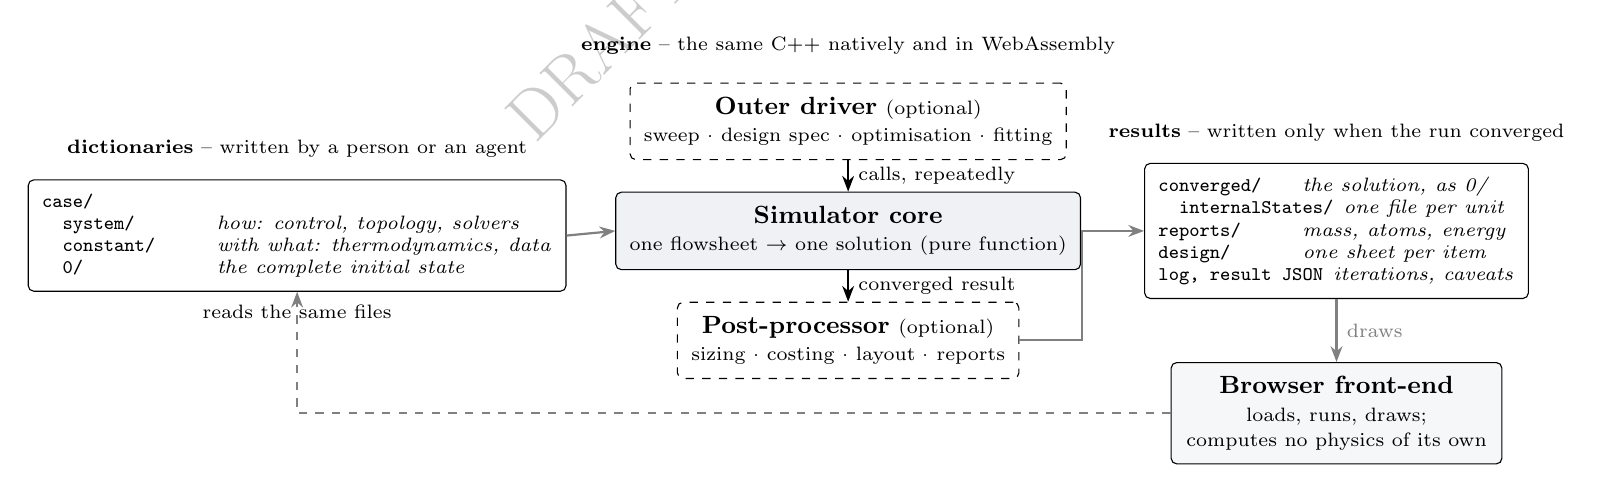
\begin{tikzpicture}[
    box/.style={draw, rounded corners=2pt, align=center, font=\small,
                inner sep=5pt},
    lay/.style={box, minimum width=4.2cm, minimum height=0.85cm},
    opt/.style={lay, dashed},
    arr/.style={-{Stealth[length=2mm]}, thick},
    node distance=0.4cm]
  % the dictionaries
  \node[draw, rounded corners=2pt, align=left, font=\scriptsize\ttfamily,
        inner sep=5pt] (case) {%
    case/\\
    \ \ system/\ \ \ \ \ \ \ \ \textrm{\itshape how: control, topology, solvers}\\
    \ \ constant/\ \ \ \ \ \ \textrm{\itshape with what: thermodynamics, data}\\
    \ \ 0/\ \ \ \ \ \ \ \ \ \ \ \ \ \textrm{\itshape the complete initial state}};
  \node[font=\scriptsize, align=center, above=0.15cm of case]
    {\textbf{dictionaries} -- written by a person or an agent};
  % the engine
  \node[opt, right=0.8cm of case, yshift=1.45cm] (outer)
    {\textbf{Outer driver} \scriptsize(optional)\\[-1pt]
     \scriptsize sweep · design spec · optimisation · fitting};
  \node[lay, below=of outer, fill=linkink!7] (core)
    {\textbf{Simulator core}\\[-1pt]
     \scriptsize one flowsheet $\rightarrow$ one solution (pure function)};
  \node[opt, below=of core] (post)
    {\textbf{Post-processor} \scriptsize(optional)\\[-1pt]
     \scriptsize sizing · costing · layout · reports};
  \draw[arr] (outer) -- node[right, font=\scriptsize]{calls, repeatedly} (core);
  \draw[arr] (core) -- node[right, font=\scriptsize]{converged result} (post);
  \node[draw=none, fit=(outer)(core)(post), inner sep=6pt] (engine) {};
  \node[font=\scriptsize, align=center, above=0.02cm of engine]
    {\textbf{engine} -- the same C++ natively and in WebAssembly};
  \draw[arr, gray] (case.east) -- (core.west);
  % the results
  \node[draw, rounded corners=2pt, align=left, font=\scriptsize\ttfamily,
        inner sep=5pt, right=0.8cm of core] (res) {%
    converged/\ \ \ \ \textrm{\itshape the solution, as 0/}\\
    \ \ internalStates/\ \textrm{\itshape one file per unit}\\
    reports/\ \ \ \ \ \ \textrm{\itshape mass, atoms, energy}\\
    design/\ \ \ \ \ \ \ \textrm{\itshape one sheet per item}\\
    log, result JSON\ \textrm{\itshape iterations, caveats}};
  \node[font=\scriptsize, align=center, above=0.15cm of res]
    {\textbf{results} -- written only when the run converged};
  \draw[arr, gray] (post.east) -| ($(post.east)!0.5!(res.west)$) |- (res.west);
  % the GUI
  \node[box, below=0.8cm of res, minimum width=4.2cm, fill=linkink!4] (gui)
    {\textbf{Browser front-end}\\[-1pt]
     \scriptsize loads, runs, draws;\\[-2pt]
     \scriptsize computes no physics of its own};
  \draw[arr, gray] (res.south) -- node[right, font=\scriptsize]{draws} (gui.north);
  \draw[arr, gray, dashed] (gui.west) -| ($(case.south)+(0,-0.3)$) -- (case.south);
  \node[font=\scriptsize, below=0.05cm of case, xshift=0.0cm, align=center]
    {reads the same files};
\end{tikzpicture}
}}}
\caption{Dictionaries, engine, results and front-end.  The three layers of
the engine; dashed layers are optional.  The browser front-end runs the
same compiled engine and draws what it published.}
\label{fig:arch}
\end{figure}

The engine has three layers (Figure~\ref{fig:arch}).  The simulator core
maps one flowsheet to one solution as a pure function of its inputs.  An
optional outer driver calls that function repeatedly (sweeps, design
specifications, optimisation, parameter estimation), and an optional
post-processor chain adds sizing, costing and layout.  Numerical strategies
coexist in each binary and are chosen in the case: Newton and Wegstein
\citep{wegstein1958} on declared tear streams, Nelder--Mead
\citep{nelder1965}, Levenberg--Marquardt \citep{marquardt1963}, Michelsen's
stability test \citep{michelsen1982}, explicit and Rosenbrock integrators.
Every extensible base class (unit operations, thermodynamic models, drivers,
sizers) has a factory, and every built-in type is registered by one line in
a function \code{main()} calls explicitly, so the origin of a model is one
readable function.  A user may add a unit operation or a rate law by the
same mechanism, compiled into a per-case binary on a local installation,
or write a rate law as a dimension-checked formula in the case file.  The
browser front-end runs the same C++ compiled to WebAssembly; it loads the
dictionaries, runs the engine and draws what the engine published, and
computes no equilibrium, balance or size itself.
% CLAUDE.md sec 4 (three layers; runSimulation the pure function), sec 5
% (factories, registerBuiltins), sec 6 "A CASE CARRIES ITS OWN KINETICS"
% (core/Formula, the expression route), sec 12 (the GUI is a viewer);
% src/solver/ (NewtonND, Wegstein, NelderMead, StabilityTest, ODE/).

\paragraph{\OF}  The case organisation (\code{system/}, \code{constant/},
\code{0/}, keyword--value dictionaries, time directories) follows
\OF\textsuperscript{\textregistered}\footnote{OPENFOAM\textsuperscript{\textregistered}
is a registered trade mark of OpenCFD Limited, producer and distributor of
the OpenFOAM software via www.openfoam.com.} \citep{weller1998}; the main
departures are one binary per problem class rather than per algorithm,
explicit registration instead of registration macros, and mandatory units
on every dimensional value.  \textbf{Choupo is an independent project: it
is not part of, affiliated with, endorsed by or sponsored by OpenCFD Ltd
or the OpenFOAM Foundation, and no \OF\ source code was adapted or reused
in it.}  \emph{This offering is not approved or endorsed by OpenCFD
Limited, producer and distributor of the OpenFOAM software via
www.openfoam.com, and owner of the OPENFOAM\textsuperscript{\textregistered}
and OpenCFD\textsuperscript{\textregistered} trade marks.}
% OpenCFD's Trade Mark Policy (read 2026-10-21; points 3, 4, 11); NOTICE
% (provenance review: independent implementations).  The long comparison
% table of revision 1 was cut (review point 9).

%===============================================================================
\section{Verification and validation: the method}
\label{sec:vv}

\subsection{Three questions kept apart}
\label{sec:vv-three}

A run answers three different questions, and Choupo reports each
separately.
\begin{description}[leftmargin=1.4em, itemsep=2pt]
\item[Numerical convergence] -- did the iteration meet its declared
  criterion?  Each solver declares a tolerance, a relative tolerance and an
  iteration limit; convergence is decided on a normalised residual (one
  home, \code{solver/Convergence.H}) and the run prints the raw and
  normalised residuals and the criterion that decided.  \code{converged/}
  is written only when the steady solve converged, and means exactly this
  and nothing more.
\item[Physical consistency] -- does the converged answer conserve mass,
  atoms and energy?  Three balances are computed after the solve, from the
  stream states, by the reporting layer (Section~\ref{sec:vv-balances}), and
  printed whether or not the case asked for them.  A converged run may be
  inconsistent, and the balance report is how a user sees it: the earlier
  draft of this paper showed a converged Cavett plant whose first law missed
  by 88~\% (Section~\ref{sec:ex-recycle}).
\item[Acceptance] -- is the answer right for its purpose?  That needs an
  independent reference: a measurement, a published solution, a hand
  calculation.  A regression pass does not answer it (below).
\end{description}
% src/solver/Convergence.H (tolerance, relTol, maxIter; normFactor);
% CLAUDE.md sec 6 "NORMALIZED RESIDUAL"; main.cpp writeConverged only when
% result.converged; the balance reports: src/reporting/.

\subsection{The balances, their normalisation and their tolerances}
\label{sec:vv-balances}

For a plant with boundary inlets $\mathcal{I}$ and outlets $\mathcal{O}$
(streams internal to the flowsheet excluded) the reports compute
\begin{align}
\text{mass closure} &= 100\,\frac{\sum_{s\in\mathcal{O}} \dot m_s}
                                    {\sum_{s\in\mathcal{I}} \dot m_s}\ \%,
\qquad
\text{element closure}_e = 100\,\frac{\sum_{s\in\mathcal{O}} \dot n_{e,s}}
                                    {\sum_{s\in\mathcal{I}} \dot n_{e,s}}\ \%,
\label{eq:mass}\\
r_E &= \Big(\sum_{s\in\mathcal{I}} \dot H_s + Q + W\Big)
       - \sum_{s\in\mathcal{O}} \dot H_s,
\label{eq:energy}\\
\varepsilon_E &= 100\,\frac{r_E}{\max\big(\sum_u |Q_u| + \sum_u |W_u|,\ |Q|\big)}\ \%,
\label{eq:energypct}
\end{align}
where $\dot H_s$ is each stream's enthalpy on the elements-and-formation
datum, priced by the thermodynamic model of the unit it leaves after
resolving its phase split, $Q$ and $W$ are the heat and shaft work crossing
the boundary, and the denominator is the energy the plant
\emph{exchanges}.  Dividing by the enthalpy throughput instead, which is
dominated by the formation datum passing through unchanged, made a real
gap look small; dividing by the terms the equation balances is the same
rule the solver uses for its residuals.  When a plant declares no duty and
no work, the denominator vanishes, and the report prints the residual in
kW with the statement that no percentage exists.  The same report prints
each unit's own residual, so a plant-level gap is localised.
% src/reporting/ (globalEnergyBoundary: residual_basis "energy exchanged
% (the larger of: sum of |declared duties and work|, and |Q boundary|)",
% read in every globalEnergyBoundary.csv of this revision's runs);
% CLAUDE.md sec 6, 2026-09-25 ("normalise by THE TERMS THE EQUATION
% BALANCES"); flashState::priceState (StreamEquilibrium.H).

Two automated checks read these reports on every steady case of the corpus
and never recompute them: mass closure within $100\pm0.5$~\%, and
$|\varepsilon_E|\le 1$~\% or, where no percentage exists,
$|r_E|\le 1$~kW.  These numbers are detection thresholds, not accuracy
claims, and they are conventions: a plant with recycles converges its tear
streams to a declared relative tolerance (typically $10^{-6}$), so it
closes to a residual and not to zero, and the thresholds are the loosest
values that are still a physical statement while sitting three or more
orders of magnitude above what a converged tear explains.  A plant losing
0.4~\% of its mass passes; the defect the mass check was built for created
13~\%.  Plants known not to close are listed by name with their measured
residual, and a listed residual that grows by more than 0.2 percentage
points, changes sign, or closes without the list being updated fails the
check, so that the list keeps describing the engine as it is.
Table~\ref{tab:coverage} reconciles the coverage.
% bin/curate/check_mass_closure.py:20-29 ("WHY A BAND AND NOT MACHINE ZERO";
% the 113 % defect), BAND = 0.5 (:141); bin/curate/check_energy_closure.py:
% 401-428 (BAND 1.0 "NOT derived from anything"; BAND_KW 1.0 "a DECLARED
% CONVENTION with no physical basis"; RATCHET 0.2).

\begin{table}[t]
\centering\scriptsize
\caption{Coverage of the two conservation checks over the 286 steady cases
of the corpus (494 cases in all; the other 208 are batch, dynamic and
property cases, whose balances are held by other checks or not at all).
Each count is the check's own claim line on the tree of this revision.}
\label{tab:coverage}
\begin{tabular}{p{8.4cm}rr}
\toprule
& \textbf{mass} & \textbf{energy} \\
\midrule
close within the threshold (energy: in \%, or in kW where no \% exists)
  & 261 & 113 + 71 \\
listed by name as not closing (residual pinned) & -- & 5 + 7 \\
balance refused for want of an enthalpy datum on a boundary stream
  & -- & 70 \\
no material boundary (closed cycles) & 4 & -- \\
report did not run under an outer driver (announced) & 1 & 1 \\
no report of that kind printed & 13 & 13 \\
exit non-zero (held by the suite's exit-code check) & 7 & 7 \\
\midrule
total & 286 & 287$^{a}$ \\
\bottomrule
\multicolumn{3}{p{12.6cm}}{\footnotesize $^{a}$The ``listed'' row of the
energy column is the length of the check's two lists (5 + 7), so one listed
plant is also counted in another category of this pass; the column sums to
287 for 286 cases.}
\end{tabular}
\end{table}
% generated/gateManifest.json (3e5d03c52) claims of check_mass_closure and
% check_energy_closure, and their re-run on this tree (supplement S1): the
% manifest at 3e5d03c52 said 255 for mass; the re-run says 261 (286 in all).

\paragraph{Independent checks of the reports}  The balance reports are
themselves code, so a few were checked by hand.  The opening flash
(Listing~\ref{lst:case}) is fed at its own temperature and pressure and
exchanges no heat, so its zero energy residual tests nothing; its
equilibrium can be tested instead: an independent bisection of the
Rachford--Rice equation on the case's own Antoine constants gives
$V/F = 0.30398357$, the engine's fourth Newton iterate.  A heater is the
smallest non-trivial energy test: 100~kW into 100~kmol/h of equimolar
ethanol and water with constant liquid heat capacities of 112.3 and
75.5~J\,mol$^{-1}$K$^{-1}$ (ideal liquid) gives
$T_\text{out} = 300 + 3600/93.9 = 338.33866$~K by hand; the engine
publishes 338.3386581~K and a first-law residual of 0.000000~kW over
100~kW exchanged.  Mass and element closures are checked the same way on
the flash, where $z_i = (1-V)x_i + V y_i$ holds to the six printed digits.
These are verification of the arithmetic, not validation of the models.
% Bisection: scratch Python on log10(Psat/bar) = A - B/(T + C), benzene
% (4.01814, 1203.835, -53.226), toluene (4.07827, 1343.943, -53.773),
% z = (0.4, 0.6), T = 370 K, P = 1 bar -> V = 0.30398357314;
% engine iterate 3 V = 0.30398357 (flash01 log on this tree).  Heater:
% tutorials/steady/heat/hx01_heater run on this tree:
% converged/hotStream T 338.3386581 K; reports/balances/
% globalEnergyBoundary.csv residual 0.000000, denom 100.0000 kW; liquid Cp
% from its constant/components/{ethanol,water}.dat (112.3, 75.5).

\subsection{Regression is not validation}
\label{sec:vv-golden}

Of the 494 cases, 477 carry a reference answer that an earlier Choupo run
recorded; each suite run compares every case with it and screens every
case for NaN and infinity.  A pass proves that an answer has not moved,
not that it is right; a re-recorded reference is therefore listed row by
row, each with the reason it moved, before anything is re-recorded.  A
regression check protects the behaviour and the conditions it exercises,
and no more: a case the suite does not run, or a condition no case
reaches, is outside it.  Following the distinction of
\citet{oberkampf2010} and NASA-STD-7009 \citep{nasa7009}, validation is
a separate, named subset of cases anchored to independent published
results -- the Williams--Otto reactor \citep{williams1960}, the
IAPWS-IF97 verification tables \citep{wagner2000}, the Hamer--Wu
activity coefficients \citep{hamer1972}, a measured calcite pH
\citep{plummer1982} and others; a case whose anchor is its own training
data is labelled fit-consistency and not counted.  The membrane and
electrodialysis comparisons of Section~\ref{sec:ex-research} are with
measurements but are not yet in the named subset.  The subset holds no
rigorous column, recycle plant or liquid--liquid flowsheet anchored to a
measurement.
% generated/releaseInventory.json (3e5d03c52): 494 / 477; CLAUDE.md sec 10
% "A GOLDEN RE-RECORD IS A CLAIM"; docs/architecture/
% verification-and-validation.md sec 3; check_validation_subset claim.

\subsection{Refusal by name}
\label{sec:vv-refusal}

An input the engine cannot honour is refused before anything is computed,
with the accepted alternatives or the remedy.  Three classes are refused
this way: a word the engine dispatches on and does not know (one function
lists the accepted words and the closest match); an input that
over-specifies the problem, such as a mixture stream with a temperature, a
pressure and a vapour fraction (Listing~\ref{lst:refusal}); and an
approximation the case did not authorise, such as a missing binary pair
silently replaced by ideal behaviour, in the activity models where this
decision is wired.  Each class is held by an automated check that builds
the offending input and requires the refusal and its wording.  When a
class of error has reached a user before such a check existed, the check
was written afterwards and verified by reintroducing the defect;
Appendix~\ref{app:gates} lists the checks behind the examples of this
paper.  A check protects the conditions it exercises; it does not make a
class of error impossible.
% src/core/RegistryRefusal.H (the one home); CLAUDE.md sec 3 "A STREAM IS
% FIXED BY TWO VARIABLES" (check_overspecified_stream); sec 6 "THE PROBLEM
% SOLVED IS NOT ALWAYS THE PROBLEM POSED" (check_problem_divergence: "NOT
% covered: only shortcutColumn and the three pair-parameter activity models
% are wired").  Revision 1 said a class "cannot come back without a test
% failing"; review point 7 -- withdrawn.

%===============================================================================
\section{Thermophysical data curation}
\label{sec:data}

\subsection{A source and a licence for every value}

Each record in the curated catalogue cites the primary source of each
value and how it was obtained (measured, regressed, estimated); a record
not yet reviewed, or read from the user's private tier, is announced each
time a run reads it.  Licence classes are decided before a value enters
the tree: a dataset with no licence statement is treated as no-grant and
kept out, as is a NonCommercial grant.  Four records whose source has an
encumbered licence are not yet replaced; they are listed by name by the
licence check rather than kept silently, so the catalogue's claim is
``a source and a licence for every value, except four listed records''.
% CLAUDE.md sec 10 licence policy; sec 7; check_source_licence claim
% (3e5d03c52): "no encumbered source stands as the authority for a value,
% except 4 pinned violations awaiting curation".  Review point 10.

\subsection{The acceptance rule}
\label{sec:accept}

A regressed parameter set (for example the two parameters of an NRTL
pair) is fitted on one study, the \emph{fit set}, and scored on a study
from another laboratory, the \emph{held-out set}, by the mean absolute
deviation of the predicted bubble temperatures,
$\mathrm{AAD} = n^{-1}\sum_i |T_i^\text{model} - T_i^\text{exp}|$.  The
set is accepted when
\begin{equation}
\mathrm{AAD} \;\le\; b \;=\; \max_i U_{95,i} \;+\; \max\big(|\delta_1|,\,|\delta_2|\big),
\label{eq:band}
\end{equation}
with $U_{95,i}$ the expanded uncertainty (95~\% coverage) the archive
states for point $i$ of the held-out set, and $\delta_1,\delta_2$ the
error of the catalogue's vapour-pressure model at the two pure-component
ends, measured with no pair involved.  The band is declared, in the case
file, before the fit is run, which prevents choosing it after seeing the
residuals; that alone does not make it adequate, so we state its basis.

If the model were exact and the measurements carried only random error
with standard uncertainty $u_i = U_{95,i}/2$ (coverage factor 2,
\citet{jcgm2008}), the expected AAD would be
$\sqrt{2/\pi}\,\bar u \approx 0.4\,\bar U_{95}$, well below the first term
of $b$.  A pure-component vapour-pressure error enters a nearly ideal
bubble temperature approximately as $x_1\delta_1 + x_2\delta_2$, whose
magnitude never exceeds $\max(|\delta_1|,|\delta_2|)$.  The rule therefore
bounds noise and a systematic endpoint error by worst-case
\emph{linear} addition; it is conservative for a correct model and
designed not to reject one.  Its limitations are stated rather than
hidden: the archive's combined expanded uncertainties are taken as given,
and whether each source article included the propagated composition and
pressure uncertainties in them was not checked; systematic errors other
than the endpoints' (in the composition analysis, for instance) are not
modelled; and a threshold on a mean cannot see a set that fails at a few
points.  For this reason the verdict is also reported against a
$\chi^2$ statistic, $\chi^2 = \sum_i (r_i/u_i)^2$ with $n$ degrees of
freedom, which uses every point's own uncertainty.
% The rule: tutorials/props/curation/curate05_nrtl_acetone_methanol/
% system/propsDict:100-101 ("the held-out set's largest stated expanded
% uncertainty (U95 = 0.11 K) plus the catalogue vapour-pressure model's own
% error at that set's pure endpoints (methanol -0.045 K, acetone +0.024 K)
% ... = 0.0469 %, rounded UP"): b = 0.11 + max(0.045, 0.024) = 0.155 K.
% Uncertainty kind: constant/experiments/acetone-methanol-bubble-je0603170.dat
% `kind expandedCombined; level 95;` (ThermoML nCombExpandUncertValue).
% Review point 5.

\subsection{A worked example: a candidate that fails}
\label{sec:worked}

The acetone + methanol pair is the azeotrope a student meets in two plants
of the corpus, and the one of the regressed pairs that failed.  An agent
located two isobaric studies in the NIST/TRC ThermoML archive
\citep{frenkel2003}, one at 101.3~kPa \citep{chen2015} and one at 100~kPa
\citep{orchilles2007}, from two laboratories with no author in common,
extracted each with its per-point uncertainty, set the pure ends aside,
and wrote a case declaring the larger study as the fit set, the other as
held out, two NRTL parameters ($\alpha$ fixed at 0.30), uncertainty
weighting, and the band of Eq.~\eqref{eq:band}: 0.155~K (0.047~\% of the
held-out mean temperature).  The engine records the datasets with DOI,
archive file, checksum and review status, freezes a fingerprint of the
partition before the regression, fits by Levenberg--Marquardt from two
starts, and computes the verdict; it also runs bubble-point scans with
ideal behaviour, UNIFAC \citep{fredenslund1975} and the fitted NRTL
\citep{renon1968} at each study's pressure (Figure~\ref{fig:fit}).

\begin{figure}[t]
\centering
% Data: paper/whitepaper/data/*.csv, the curate05 run's outputs; re-run on
% this tree: every CSV byte-identical (cmp), log "Final chi2 4.45237e+00",
% "AAD 0.0960 % (0.3160 K)", "maxAAD 0.0470 %", "notValidated"; overlays
% txy_unifac 0.0408 K held-out / 0.3404 K fit set; txy_nrtl 0.3160 / 0.1010 K.
\pgfplotsset{every axis/.append style={font=\scriptsize, tick label style={font=\scriptsize}}}
\begin{tikzpicture}
\begin{groupplot}[group style={group size=2 by 2, horizontal sep=1.3cm,
                   vertical sep=0.55cm, x descriptions at=edge bottom},
                  width=7.4cm]
  \nextgroupplot[height=4.6cm, ylabel={$T_\mathrm{bubble}$ [K]},
                 title={\textbf{Fit study}, 101.3 kPa, 32 points},
                 ymin=327, ymax=338.5, xmin=0, xmax=1,
                 legend style={at={(0.97,0.97)}, anchor=north east, font=\tiny,
                               draw=none, fill=none}, legend cell align=left]
    \addplot[idealink, densely dotted, thick] table[col sep=comma, x index=0, y index=1]
      {\datadir/txy_ideal_fitP.csv};
    \addlegendentry{ideal}
    \addplot[unifacink, dashed, thick] table[col sep=comma, x index=0, y index=1]
      {\datadir/txy_unifac_fitP.csv};
    \addlegendentry{UNIFAC (not fitted here)}
    \addplot[fitink, thick] table[col sep=comma, x index=0, y index=1]
      {\datadir/txy_nrtl_fitP.csv};
    \addlegendentry{NRTL, fitted here}
    \addplot[only marks, mark=square*, mark size=1.6pt, fitink]
      table[col sep=comma, x index=0, y index=1] {\datadir/exp_fitset_acetone_methanol.csv};
    \addlegendentry{measured, fit set}
  \nextgroupplot[height=4.6cm,
                 title={\textbf{Held-out study}, 100 kPa, 30 points},
                 ymin=327, ymax=338.5, xmin=0, xmax=1,
                 legend style={at={(0.97,0.97)}, anchor=north east, font=\tiny,
                               draw=none, fill=none}, legend cell align=left]
    \addplot[idealink, densely dotted, thick] table[col sep=comma, x index=0, y index=1]
      {\datadir/txy_ideal.csv};
    \addlegendentry{ideal}
    \addplot[unifacink, dashed, thick] table[col sep=comma, x index=0, y index=1]
      {\datadir/txy_unifac.csv};
    \addlegendentry{UNIFAC (not fitted here)}
    \addplot[fitink, thick] table[col sep=comma, x index=0, y index=1]
      {\datadir/txy_nrtl.csv};
    \addlegendentry{NRTL, fitted on the left}
    \addplot[only marks, mark=o, mark size=1.7pt, heldink, thick]
      table[col sep=comma, x index=0, y index=1] {\datadir/exp_heldout_acetone_methanol.csv};
    \addlegendentry{measured, held out}
  \nextgroupplot[height=3.6cm, xlabel={$x_\mathrm{acetone}$},
                 ylabel={$T_\mathrm{model}-T_\mathrm{exp}$ [K]},
                 ymin=-0.6, ymax=1.0, xmin=0, xmax=1, ytick={-0.4,0,0.4}]
    \addplot[black!60, thin] coordinates {(0,0) (1,0)};
    \addplot[only marks, mark=square*, mark size=1.5pt, fitink]
      table[col sep=comma, x index=0, y index=4] {\datadir/parity.csv};
    \node[font=\tiny, anchor=south west, align=left] at (axis cs:0.02,0.62)
      {NRTL on its own fit set: AAD 0.10 K};
  \nextgroupplot[height=3.6cm, xlabel={$x_\mathrm{acetone}$},
                 ymin=-0.6, ymax=1.0, xmin=0, xmax=1, ytick={-0.4,0,0.4},
                 legend style={at={(0.03,0.97)}, anchor=north west, font=\tiny,
                               draw=none, fill=none}, legend cell align=left,
                 legend columns=1]
    \addplot[black!60, thin, forget plot] coordinates {(0,0) (1,0)};
    \addplot[only marks, mark=o, mark size=1.6pt, fitink, thick]
      table[col sep=comma, x index=0, y index=2] {\datadir/heldout_residuals.csv};
    \addlegendentry{NRTL: AAD 0.316 K, $\chi^2$ 1935}
    \addplot[only marks, mark=triangle, mark size=1.7pt, unifacink, thick]
      table[col sep=comma, x index=0, y index=3] {\datadir/heldout_residuals.csv};
    \addlegendentry{UNIFAC: AAD 0.041 K, $\chi^2$ 31}
\end{groupplot}
\end{tikzpicture}
\caption{The acetone + methanol regression, drawn from the run's files.
Top: bubble-point curves at each study's pressure, with the fit study
(left) and the held-out study (right).  Bottom: residuals per point.  The
acceptance criterion applies to the \emph{mean} absolute residual (AAD),
not to individual points: the band declared before the fit is
$b = 0.155$~K; the held-out points carry stated expanded uncertainties of
0.09--0.11~K each.  $\chi^2$ is $\sum (r_i/u_i)^2$ with $u_i = U_{95,i}/2$
over the 30 held-out points; its 95~\% quantile is 43.8.  The fitted pair
reproduces its own study and fails the other (verdict
\texttt{notValidated}); UNIFAC does the mirror image.}
\label{fig:fit}
\end{figure}
% chi2: scratch Python on paper/whitepaper/data/heldout_residuals.csv with
% the held-out file's U95 values (0.11 0.11 0.1 0.1 0.1, then 0.09 x 25):
% NRTL 1935.4, UNIFAC 31.4, ideal 1.41e5; expected AAD for noise alone
% sqrt(2/pi) mean(u) = 0.037 K.  chi2_{0.95}(30) = 43.77 (tables).

The fitted pair reproduces its own study to 0.10~K and misses the
held-out study by 0.316~K, twice the band: the verdict is
\code{notValidated} and the pair does not enter the catalogue.  The
verdict does not depend on the details of the rule: against the per-point
uncertainties the held-out residuals give $\chi^2 = 1935$ on 30 points
(95~\% quantile 43.8), and noise alone would give an AAD of about
0.037~K.  UNIFAC reproduces the held-out study to 0.041~K ($\chi^2 = 31$,
consistent with the stated uncertainties) and misses the fit study by
0.34~K.  UNIFAC was not fitted to either study \emph{in this work}; its
group parameters were regressed by their authors to a large VLE database
that may include data for this binary, so its agreement is not evidence
of independence.  The two studies disagree with each other by about
0.3~K where each states 0.1--0.35~K, so at least one carries an error its
uncertainty does not describe; which one is a question for a curator who
reads both articles, and neither dataset has yet been read back against
its article (the archive transcription was used; every run says so).
For a column at these pressures both models place the azeotrope near
$x_\text{acetone}\approx 0.78$ at 100~kPa; we do not claim that a column
design is insensitive to the choice, which depends on the equilibrium
along the whole column and on how close the specification is to the
azeotrope.  A second candidate fails the other way: an ethanol +
cyclohexane pair passed its held-out band and was not promoted, because
it predicts two liquids across its validity span where both studies
report one -- a bubble-temperature test solves for one liquid by
construction and cannot see a second, so acceptance also requires a
stability scan.
% curate05 run (this tree); curate12 run (this tree): verdict validated;
% check_regressed_pairs claim (arm f: one liquid across the span).  The
% reviewer's objection to "the column design is not sensitive" (point 4)
% -- withdrawn.  Read-back of the articles: TODO B10.

%===============================================================================
\section{Results}
\label{sec:examples}

Every number in this section was read from a run of a named case on the
tree of this revision; supplement S1 lists the commands.

\subsection{A flash and a refusal}
\label{sec:ex-simple}

Listing~\ref{lst:log} is an excerpt of the run log of the flash of
Listing~\ref{lst:case}.  It prints the model, the vapour pressures and
$K$-values, each Newton iteration of the Rachford--Rice equation, that
benzene's vapour pressure was evaluated outside the range of its Antoine
correlation, and at the end every assumption the run raised.  A stream of
known component flows is fixed by two intensive variables; the same feed
given a vapour fraction as well is refused before any computation
(Listing~\ref{lst:refusal}).
% flash01 run on this tree: the listing lines are identical to revision 1's
% (log lines 38-131).  flash01v: vaporFraction 0.3 appended, exit 2
% (re-run on this tree: the quoted clauses are verbatim from its log;
% check_overspecified_stream holds the refusal).

\Needspace{18\baselineskip}
\begin{lstlisting}[caption={Excerpt of the run log of the flash
  (\texttt{verbosity 3}); elided lines marked \texttt{[...]}.},label=lst:log,
  breaklines=true, breakindent=0pt]
>>>  Unit [0]:  flash01   (type = isothermalFlash)
>>>  thermo: inherited (global package)
  [flash] model rachfordRice  (declared)
[psat] component 'benzene': Antoine evaluated at T = 370 K, OUTSIDE its declared Trange (287.7 354.07).
K-values  (γ = ideal,  φ = idealGas,  evaluated at x = z initially):
  benzene       Psat = 1.6514 bar    K = 1.6514
  toluene       Psat = 0.6735 bar    K = 0.6735
  [outer 0] Rachford-Rice Newton (inner):
    it          V           g(V)         dg/dV         ΔV
    0     0.50000000   -3.75806e-02   -1.87920e-01   -1.99981e-01
    1     0.30001863   7.81978e-04    -1.97366e-01   3.96206e-03
    2     0.30398070   5.66359e-07    -1.97081e-01   2.87374e-06
    3     0.30398357   2.94959e-13    -1.97081e-01   0.00000e+00
[...]
  V/F:           0.303984
  Component         z          x          y          K
  benzene         0.400000  0.333888  0.551373    1.6514
  toluene         0.600000  0.666112  0.448627    0.6735
[...]
PROBLEM SOLVED == PROBLEM POSED.  No divergence declared or imposed.
ASSUMPTIONS AND CAVEATS -- what this run announced along the way
  EXTRAPOLATIONS AND VALIDITY  (3)
    - component 'benzene': vapour pressure evaluated at T = 370 K, OUTSIDE its declared Trange (287.7 354.07) -- extrapolated, still returned
\end{lstlisting}

\Needspace{10\baselineskip}
\begin{lstlisting}[caption={A refusal by name (the feed of
  Listing~\ref{lst:case} with \texttt{vaporFraction 0.3;} added); exit
  status 2.},label=lst:refusal, breaklines=true, breakindent=0pt]
ERROR: stream state 'feed': OVER-SPECIFIED -- declares T = 370 K, P = 100000 Pa AND vaporFraction = 0.3 for a MIXTURE of 2 components (benzene, toluene).  A stream of known component flows is fixed by TWO intensive variables (Duhem's theorem); [...] Remedies: (1) delete the `vaporFraction` line and let (T, P) resolve the split [...]; (2) if the QUALITY is the specification, the state is (P, q) or (T, q) and the other variable must be SOLVED from it [...].
\end{lstlisting}

\subsection{An integrated process with recycles: the Cavett problem}
\label{sec:ex-recycle}

The Cavett problem \citep{cavett1963} is a classical recycle benchmark:
four flash drums at 800, 270, 49 and 13~psia, two mixers, three recycle
streams (one liquid, two vapours) and a sixteen-component feed of
27\,340.6~kmol/h entering the second stage (Figure~\ref{fig:cavett}).  The
case runs it on the specification of \citet{rosen1977} with SRK
\citep{soave1972}, every $k_{ij}$ zero and declared, the mixers adiabatic,
and Newton on the two mixer outlets as tear streams.
% tutorials/steady/flowsheets/cavett01_recycle_train: system/flowsheetDict
% (FL1..FL4 at 310.928 K/55.1581 bar, 322.039/18.6159, 308.706/3.3784,
% 302.594/0.8963; M2 inputs feed L1 V3, M3 inputs L2 V4; mixers declare no
% T, i.e. adiabatic), system/solverDict (tearStreams mixed2 mixed3,
% recycleTol 1e-6, Newton).

\begin{figure}[t]
\centering
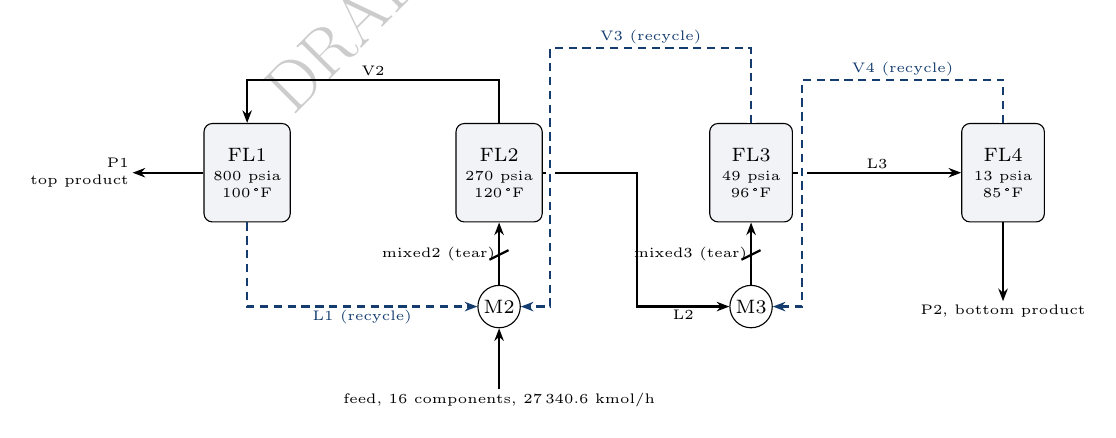
\begin{tikzpicture}[
    fl/.style={draw, rounded corners=3pt, minimum width=1.05cm,
               minimum height=1.25cm, align=center, font=\scriptsize,
               fill=linkink!6},
    mx/.style={draw, circle, inner sep=1.2pt, font=\scriptsize, fill=white},
    st/.style={-{Stealth[length=1.6mm]}, thick},
    rc/.style={st, densely dashed, linkink},
    halo/.style={preaction={draw=white, line width=3.2pt}},
    lab/.style={font=\tiny, inner sep=1pt}]
  \node[fl] (F1) at (0,0)    {FL1\\[-1pt]\tiny 800 psia\\[-2pt]\tiny 100\,\textdegree F};
  \node[fl] (F2) at (3.2,0)  {FL2\\[-1pt]\tiny 270 psia\\[-2pt]\tiny 120\,\textdegree F};
  \node[fl] (F3) at (6.4,0)  {FL3\\[-1pt]\tiny 49 psia\\[-2pt]\tiny 96\,\textdegree F};
  \node[fl] (F4) at (9.6,0)  {FL4\\[-1pt]\tiny 13 psia\\[-2pt]\tiny 85\,\textdegree F};
  \node[mx] (M2) at (3.2,-1.7) {M2};
  \node[mx] (M3) at (6.4,-1.7) {M3};
  % feed and products
  \draw[st] (3.2,-2.75) node[below, lab] {feed, 16 components, 27\,340.6 kmol/h} -- (M2.south);
  \draw[st] (F1.west) -- ++(-0.9,0) node[left, lab, align=right] {P1\\top product};
  \draw[st] (F4.south) -- ++(0,-1.0) node[below, lab] {P2, bottom product};
  % tears
  \draw[st] (M2.north) -- node[left, lab, pos=0.5] {mixed2 (tear)} (F2.south);
  \draw[st] (M3.north) -- node[left, lab, pos=0.5] {mixed3 (tear)} (F3.south);
  \foreach \m in {M2, M3}
    \draw[thick] ($(\m.north)+(-0.12,0.32)$) -- ++(0.24,0.12);
  % vapour up the cascade, liquid down
  \draw[st] (F2.north) -- ++(0,0.55) -| node[pos=0.25, above, lab] {V2} (F1.north);
  \draw[rc] (F1.south) |- node[pos=0.75, below, lab] {L1 (recycle)} (M2.west);
  \draw[st] (F2.east) -- ++(1.2,0) |- node[pos=0.75, below, lab] {L2} (M3.west);
  \draw[rc, halo] (F3.north) -- ++(0,0.95) -| node[pos=0.25, above, lab] {V3 (recycle)} (3.85,-1.7) -- (M2.east);
  \draw[st] (F3.east) -- node[above, lab] {L3} (F4.west);
  \draw[rc, halo] (F4.north) -- ++(0,0.55) -| node[pos=0.25, above, lab] {V4 (recycle)} (7.05,-1.7) -- (M3.east);
\end{tikzpicture}

\vspace{4pt}
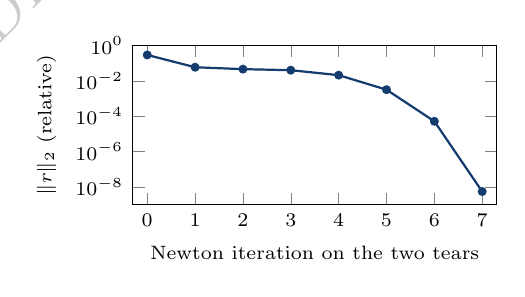
\begin{tikzpicture}
  \begin{axis}[width=6.2cm, height=3.6cm, ymode=log, font=\scriptsize,
               xlabel={Newton iteration on the two tears},
               ylabel={$\|r\|_2$ (relative)},
               xmin=-0.3, xmax=7.3, ymin=1e-9, ymax=1, xtick={0,...,7},
               ytick={1e-8,1e-6,1e-4,1e-2,1}]
    \addplot[linkink, thick, mark=*, mark size=1.2pt] coordinates
      {(0,2.927e-1) (1,5.896e-2) (2,4.601e-2) (3,4.016e-2) (4,2.101e-2)
       (5,3.161e-3) (6,5.126e-5) (7,5.393e-9)};
  \end{axis}
\end{tikzpicture}
\caption{The Cavett problem as the case declares it (top): four
isothermal flash drums, two adiabatic mixers, the two torn streams
(slashed) and the three recycles (dashed).  Bottom: the Newton history on
the tears.}
\label{fig:cavett}
\end{figure}
% The run of cavett01 on this tree: log "Recycle outer loop (Newton over 2
% tear stream(s), 34 variables)", |r|2 at it 0..6 = 2.927e-01 5.896e-02
% 4.601e-02 4.016e-02 2.101e-02 3.161e-03 5.126e-05, "Recycle converged in 7
% Newton iteration(s) (|r|2 = 5.393e-09)".

Table~\ref{tab:cavett} keeps the three questions of
Section~\ref{sec:vv-three} apart.  The run converges in seven Newton
iterations; Wegstein acceleration on the same problem limit-cycles and stops
at its iteration limit, and the run exits with status~1 and writes no
\code{converged/}.  The converged plant closes its mass balance to
100.0000~\%, every element to 0.0011~\%, and its first law to $+0.0019$~kW
of 396\,325~kW exchanged; each of the six units leaves at most 0.0025~kW
unattributed.  This is the corrected case.  In the first draft of this
paper the same plant, converged, missed its first law by $-549\,319$~kW
(88~\% of the energy exchanged), and the per-unit report put the whole gap
on the two mixers: the adiabatic mixer published its outlet in the phase
of its dominant inlet and computed its temperature on a different
enthalpy surface from the one the report prices.  The mixer now returns the
state of equal enthalpy resolved at its own phase equilibrium, priced as
the report prices it (the mixed streams flash, to 269.7 and 273.6~K), and
both mixers close to 0.0000~kW.  The earlier run is the example of the
first two questions coming apart: numerically converged, physically
inconsistent, and visibly so in the default report.
% cavett01 run: reports/balances/massBalance.csv closure_pct 100.0000 (net
% -0.3544 of 1 870 617.6 kg/h); elementBalance "worst element closure off
% by 0.0011 %"; globalEnergyBoundary.csv residual 0.001858 kW, denom
% 396324.9894 kW; energyBalance_byUnit.csv remaining_kW max |-0.0025| (FL3),
% M2 -0.0000, M3 0.0000; converged/mixed2 T 269.6666353 K, mixed3
% 273.6237673 K.  Wegstein: recycleSolver Wegstein in a scratch copy:
% "WARNING: recycle did NOT converge in 300 iterations (last |Δtear|2 =
% 2.2912e-02)", exit 1, no converged/.  Before the fix: revision 1's run
% of 2026-10-21 (residual -549319.11 kW, -88.02 % of 624070.6 kW; M2
% +352666.2, M3 +196652.9 kW).  The fix: commit 4c8a5097a ("The adiabatic
% mixer's outlet is the state of equal enthalpy, resolved at its own
% equilibrium"); DEV.md 4c 2026-10-25 "C131 phase 1 DONE".

\begin{table}[t]
\centering\scriptsize
\caption{The Cavett problem, the three questions of
Section~\ref{sec:vv-three} answered separately (the run of this revision).
Product flows are those of stream P1 (top product).}
\label{tab:cavett}
\begin{tabular}{p{3.0cm}p{5.6cm}p{5.0cm}}
\toprule
\textbf{question} & \textbf{evidence} & \textbf{verdict} \\
\midrule
numerical convergence & Newton, 7 iterations, $\|r\|_2 = 5.4\times10^{-9}$
  against $10^{-6}$; Wegstein: 300 iterations, $\|\Delta\|_2 = 2.3\times10^{-2}$
  & converged (Newton); not converged, no answer written (Wegstein) \\
physical consistency & mass 100.0000~\%; elements within 0.0011~\%;
  first law $+0.0019$~kW of 396\,325~kW exchanged & consistent \\
acceptance & P1: N$_2$ 358.2, CH$_4$ 2995.4, ethane 2383.8, isobutane
  153.9~kmol/h; FLOWTRAN \citep{rosen1977}: isobutane 198.2~kmol/h &
  agreement on the light ends; the loop intermediates differ with the
  $K$-model (SRK, $k_{ij}=0$ here); no measurement exists \\
\bottomrule
\end{tabular}
\end{table}
% converged/P1: N2 358.2003381, CH4 2995.435982, ethane 2383.817471,
% isoButane 153.8691154 kmol/h.  The FLOWTRAN values: the case header
% (system/controlDict: "isoButane in P1: 153.9 here, ... 198.2 FLOWTRAN";
% FLOWTRAN CH4 and ethane as printed there were not re-read for this
% revision -- TODO (authors): read Rosen & Pauls 1977's table and quote its
% light-end values beside ours).

\subsection{Nanofiltration of multi-ionic solutions}
\label{sec:ex-research}

The engine models a spiral-wound or flat-cell nanofiltration element as a
sequence of stations along the feed channel.  At each station a transport
law gives the ion fluxes through the membrane, a polarisation model gives
the concentrations at the membrane wall, and the water flux closes
$J_v = A_w(\Delta P - \Delta\pi)$.  Two transport laws are compared with
measurements here.

\paragraph{Solution-diffusion-electromigration (SDEM)}  Following
\citet{yaroshchuk2013}, each ion $i$ crosses the active layer (coordinate
$\xi\in[0,1]$, potential $\psi$ in units of $RT/F$) with a constant
permeance $P_i$ that already contains its partition coefficient:
\begin{equation}
j_i = -P_i\left(\frac{dc_i}{d\xi} + z_i c_i \frac{d\psi}{d\xi}\right),\qquad
\sum_i z_i c_i = 0,\qquad \sum_i z_i j_i = 0,\qquad j_i = J_v\, c_{p,i},
\label{eq:sdem}
\end{equation}
with $c_i$ the virtual concentrations (of the solution that would be in
equilibrium with each point of the layer), electroneutrality of that
virtual solution, zero electric current and the permeate composition as
the closure.  The boundary conditions are the wall concentrations at
$\xi=0$ and the permeate at $\xi=1$.  The field follows from the last two
conditions with no added parameter,
$d\psi/d\xi = -\big(\sum_i z_i j_i/P_i\big)/\big(\sum_i z_i^2 c_i\big)$;
for a single salt the system reduces exactly to $R = J_v/(J_v+P_s)$ with
the ambipolar permeance $P_s = (z_+ + |z_-|)P_+P_-/(z_+P_+ + |z_-|P_-)$.
The engine integrates Eq.~\eqref{eq:sdem} from the permeate face, where the
unknown is, towards the wall, and solves for the permeate composition by
Newton at each station.
% src/unitOperations/membrane/transport/SDEM.H (Eqs. 1-4, the field, the
% ambipolar reduction, "integrates (1)-(2) BACKWARD, from the permeate face
% toward the wall, with a fixed-step RK4", inner Newton in c_p).

\paragraph{Identifiability}  A single-salt test determines one number,
$P_s$, and not the two ion permeances: by the ambipolar relation,
$1/P_s = (z_+/P_- + |z_-|/P_+)/(z_+ + |z_-|)$ is a linear combination of
the reciprocal ion permeances.  Several salts sharing ions give a linear
system in those reciprocals; for the four salts of two cations and two
anions its rank is four only because the valences differ (with equal
valences one combination is lost).  Ion permeances are therefore not
calibrated from one salt; the source study determined them from multi-salt
experiments with traces, and the engine reproduces the study's four salt
permeances from its ion permeances to the table's rounding, which is a
consistency check and not an identification.
% The ambipolar identity: SDEM.H; check_sdem arm (b) ("reproduces all 4
% Table 1 salt permeances ... within 5 %").  Rank: rows NaCl (1/2,0,1/2,0),
% Na2SO4 (2/3,0,0,1/3), MgCl2 (0,1/3,2/3,0), MgSO4 (0,1/2,0,1/2) on
% (1/P_Na, 1/P_Mg, 1/P_Cl, 1/P_SO4); with z all 1 the rows a+c, a+d, b+c,
% b+d satisfy (a+c)-(a+d)-(b+c)+(b+d) = 0.  Revision 1's sentence that
% per-ion permeances are "calibratable from the single-salt tests
% manufacturers publish" is withdrawn (review point 6).

\paragraph{Donnan--steric pore model (DSPM-DE)}  The second law resolves the
pore: the extended Nernst--Planck flux of each ion with hindered
convection, $N_i = -P_i(dc_i/d\xi + z_i c_i\,d\psi/d\xi) + K_{c,i}J_v c_i$,
electroneutrality with the membrane's fixed charge $X_d$ at every node,
zero current, and steric, dielectric and Donnan partitions at both faces
\citep{bowen2002}, with the hindrance factors of \citet{dechadilok2006}.
The pore is discretised on 101 nodes with exponentially fitted
(Scharfetter--Gummel) fluxes \citep{scharfetter1969} and every node, the
wall and the water flux are solved together by Newton, as in the program
NanoFiltran \citep{geraldes2008}.  Against NanoFiltran, on 35 published
problems, the two programs' grid-converged permeates agree within
$7.9\times10^{-7}$ relative.  That is verification by comparison with
another code; it says nothing about either code's agreement with a
membrane.
% src/unitOperations/membrane/transport/PoreNernstPlanck.H (Eqs. 1-9, the
% flux, the grid); CLAUDE.md sec 6 "A STIFF PORE SOLVED AT ONCE";
% tutorials/props/membrane/nanofiltran_geraldesAlves2008 run on this tree
% (exit 0); check_nanofiltran_reference claim (3e5d03c52): "35 anchors ...
% agrees with NanoFiltran extrapolated within 7.9e-07 relative on all 35
% rows ... NOT CHECKED: whether NanoFiltran is right (code-to-code is not
% validation)".

\paragraph{Polarisation}  The wall concentrations come from the
multi-ionic film model of \citet{geraldes2007}: each ion has its own mass
transfer coefficient from its own diffusivity, corrected for suction, and
the ions are coupled by one interface potential fixed by electroneutrality
at the wall, with no film thickness to declare.  The data used below are
\emph{intrinsic} rejections (the authors corrected them for
polarisation), so the cases make the film negligible
($k = 10$~m\,s$^{-1}$ in the fit, $k = 1$~m\,s$^{-1}$ in the trace
probes) and compare intrinsic quantities.
% src/unitOperations/membrane/massTransfer/Polarisation (CLAUDE.md sec 6
% "THE FILM WITH A FIELD"); membrane24 propsDict residual block (k_film 10;
% `rejection intrinsic;`); check_sdem build_probe (k_film 1.0).

\paragraph{Operating conditions and data}  The measurements are those of
\citet{fdl2021} (CC~BY~4.0): an NF270 membrane in a rotating-disk cell at
20~$^\circ$C, four dominant salts (NaCl, MgCl$_2$, Na$_2$SO$_4$,
MgSO$_4$) at 0.01~mol\,L$^{-1}$ with NaNO$_3$ and NH$_4$Cl traces at
$2\times10^{-4}$~mol\,L$^{-1}$, permeate fluxes 6--56~$\mu$m\,s$^{-1}$,
intrinsic rejections read from the paper's figures with the reading error
recorded per point (the source publishes no measurement uncertainty).
% membrane24 constant/experimental/fdl2021_*.dat headers (digitised by
% bin/curate/digitise_fdl2021.py; reading error per point; "the authors
% publish no measurement uncertainty").

\begin{figure}[t]
\centering
\pgfplotsset{every axis/.append style={font=\scriptsize, tick label style={font=\scriptsize}}}
\begin{tikzpicture}
\begin{groupplot}[group style={group size=2 by 1, horizontal sep=1.6cm},
                  width=7.3cm, height=6.0cm]
  \nextgroupplot[title={(a) DSPM-DE: salt transmission},
                 xlabel={$J_v$ [$\mu$m\,s$^{-1}$]}, ylabel={intrinsic transmission $1-R$},
                 xmin=0, xmax=60, ymode=log, ymin=1e-5, ymax=1.5,
                 legend style={at={(0.5,0.02)}, anchor=south, font=\tiny, legend columns=2,
                               draw=none, fill=white, fill opacity=0.8, text opacity=1},
                 legend cell align=left]
    \addplot[only marks, mark=square*, mark size=1.4pt, fitink]
      table[col sep=comma, x=Jv, y=Texp] {\cacedata/dspmde_NaCl.csv};
    \addlegendentry{NaCl, fit}
    \addplot[fitink, thick, forget plot] table[col sep=comma, x=Jv, y=Tmod] {\cacedata/dspmde_NaCl.csv};
    \addplot[only marks, mark=triangle*, mark size=1.6pt, unifacink]
      table[col sep=comma, x=Jv, y=Texp] {\cacedata/dspmde_MgCl2.csv};
    \addlegendentry{MgCl$_2$, fit}
    \addplot[unifacink, thick, forget plot] table[col sep=comma, x=Jv, y=Tmod] {\cacedata/dspmde_MgCl2.csv};
    \addplot[only marks, mark=o, mark size=1.6pt, heldink, thick]
      table[col sep=comma, x=Jv, y=Texp] {\cacedata/dspmde_Na2SO4.csv};
    \addlegendentry{Na$_2$SO$_4$, held out}
    \addplot[heldink, thick, dashed, forget plot] table[col sep=comma, x=Jv, y=Tmod] {\cacedata/dspmde_Na2SO4.csv};
    \addplot[only marks, mark=diamond, mark size=1.8pt, black, thick]
      table[col sep=comma, x=Jv, y=Texp] {\cacedata/dspmde_MgSO4.csv};
    \addlegendentry{MgSO$_4$, held out}
    \addplot[black, thick, dashed, forget plot] table[col sep=comma, x=Jv, y=Tmod] {\cacedata/dspmde_MgSO4.csv};
  \nextgroupplot[title={(b) SDEM: trace ions on MgSO$_4$},
                 xlabel={$J_v$ [$\mu$m\,s$^{-1}$]}, ylabel={$f = 1/(1-R)$},
                 xmin=0, xmax=60, ymin=0, ymax=9.5,
                 legend style={at={(0.02,0.98)}, anchor=north west, font=\tiny,
                               draw=none, fill=white, fill opacity=0.8, text opacity=1},
                 legend cell align=left]
    \addlegendimage{only marks, mark=*, mark size=1.4pt, black}
    \addlegendentry{measured}
    \addlegendimage{gray, thin}
    \addlegendentry{authors' SDEM line}
    \addlegendimage{black, thick}
    \addlegendentry{Choupo, trace limit}
    \addlegendimage{black, thick, densely dashed}
    \addlegendentry{Choupo, $2\times10^{-4}$ M traces}
    \addplot[only marks, mark=*, mark size=1.4pt, black, forget plot]
      table[col sep=comma, x=Jv, y=fexp] {\cacedata/sdem_Na.csv};
    \addplot[gray, thin, unbounded coords=jump, forget plot]
      table[col sep=comma, x=Jv, y=fline] {\cacedata/sdem_Na.csv};
    \addplot[fitink, thick, forget plot] table[col sep=comma, x=Jv, y=ftrace] {\cacedata/sdem_Na.csv};
    \addplot[fitink, thick, densely dashed, forget plot] table[col sep=comma, x=Jv, y=fpaper] {\cacedata/sdem_Na.csv};
    \addplot[only marks, mark=*, mark size=1.4pt, black, forget plot]
      table[col sep=comma, x=Jv, y=fexp] {\cacedata/sdem_Cl.csv};
    \addplot[gray, thin, unbounded coords=jump, forget plot]
      table[col sep=comma, x=Jv, y=fline] {\cacedata/sdem_Cl.csv};
    \addplot[heldink, thick, forget plot] table[col sep=comma, x=Jv, y=ftrace] {\cacedata/sdem_Cl.csv};
    \addplot[heldink, thick, densely dashed, forget plot] table[col sep=comma, x=Jv, y=fpaper] {\cacedata/sdem_Cl.csv};
    \addplot[only marks, mark=*, mark size=1.4pt, black, forget plot]
      table[col sep=comma, x=Jv, y=fexp] {\cacedata/sdem_NO3.csv};
    \addplot[gray, thin, unbounded coords=jump, forget plot]
      table[col sep=comma, x=Jv, y=fline] {\cacedata/sdem_NO3.csv};
    \addplot[unifacink, thick, forget plot] table[col sep=comma, x=Jv, y=ftrace] {\cacedata/sdem_NO3.csv};
    \addplot[unifacink, thick, densely dashed, forget plot] table[col sep=comma, x=Jv, y=fpaper] {\cacedata/sdem_NO3.csv};
    \node[font=\tiny, fitink] at (axis cs:50,8.9) {Na$^+$};
    \node[font=\tiny, heldink] at (axis cs:57,2.95) {Cl$^-$};
    \node[font=\tiny, unifacink] at (axis cs:57,0.55) {NO$_3^-$};
\end{groupplot}
\end{tikzpicture}
\caption{NF270 \citep{fdl2021}: measurements (markers) against Choupo
(lines).  (a) DSPM-DE with its pore radius and fixed charge fitted to the
two chlorides (solid lines) and the two sulfates predicted (dashed), on the
transmission scale $1-R$; on the rejection scale the sulfate points and
lines overlap at $R \approx 0.98$--$1$.  (b)
SDEM with the paper's Table~1 permeances, trace ions on a 0.01~M MgSO$_4$
feed: Choupo in the trace limit the authors' analytical line assumes
(solid), and at the experiments' own trace concentration (dashed); the
thin grey line is the authors' own fit.}
\label{fig:nf}
\end{figure}
% (a) paper/cace/data/dspmde_*.csv, written by figures/gen_dspmde_fit.py
% (membrane24 in props mode, its default `rejections` view).
% (b) paper/cace/data/sdem_*.csv, written by figures/gen_sdem_traces.py
% (check_sdem's build_probe / run_at_flux imported; the measured symbols
% and the authors' line from membrane12's constant/experimental/
% fdl2021_figures.csv, Figure 4b).

\paragraph{Validation against measurements}  Figure~\ref{fig:nf}a is the
DSPM-DE pore fitted to the measured rejections of the two chlorides: pore
radius $0.675\pm0.034$~nm and fixed charge $-10.5\pm4.1$~mol\,m$^{-3}$
(95~\% intervals; correlation $-0.96$), and the two sulfates, never seen by
the fit, predicted with a mean absolute error of 0.93 rejection points
against the 10 points the case declared before the fit.  Two qualifications
belong with that number.  The partition into fit and held-out salts was
chosen after two others had been measured and found not identifiable (the
case says so), and held-out salts of the same study are not an independent
study.  And the sulfates' rejections are near unity, where a tight pore of
almost any charge predicts them closely: on the transmission scale, $1-R$,
the prediction is 9--12 times too low for Na$_2$SO$_4$ and 49--67 times too
low for MgSO$_4$.  The acceptance criterion measured in rejection points
is passed; on transmission it would fail.  The scale on which a membrane
model is judged is part of the claim.
% membrane24 props run on this tree: "poreModel.poreRadius = 6.7476e-10 m
% +/- 3.402e-11 (95 %)", "chargeDensity = -10.525 mol/m3 +/- 4.097e+00",
% "correlation ... = -0.9621", "HELD-OUT EVIDENCE 14 measurement(s); AAD
% 0.926 points", "maxAAD 10.000", "validated"; the partition history: the
% case's system/propsDict header ("CHOSEN AFTER MEASURING THE
% ALTERNATIVES").  Transmission ratios: scratch Python on
% data/dspmde_Na2SO4.csv (9.3-12.2) and dspmde_MgSO4.csv (48.7-66.5).

Figure~\ref{fig:nf}b separates two things the first draft blurred.  In the
trace limit, which the authors' analytical line assumes, Choupo's SDEM
reproduces that line within 3.5--5~\% on average on the three trace ions
shown, and the measurements within 7--8~\%.  At the experiments' own trace
concentration it does not: the transmission of Na$^+$ rises by a factor
of 1.5--2.3 and that of NO$_3^-$ falls by a fifth to a third, and $f$
departs from the measurements by 20--46~\% on average.  The reason is physical and is the source paper's own caveat: on
this feed a trace nitrate at $P = 42~\mu$m\,s$^{-1}$ carries more current
than 0.01~M of sulfate at $0.13~\mu$m\,s$^{-1}$, so the traces relax the
field the trace-limit solution assumes they do not touch.  The measured
points follow the trace-limit line because the permeances were fitted
\emph{with} that approximation; the full model with the same permeances
departs from the measurements.  Parameters estimated under one
approximation are not transferable to a model that drops it, and the
consistent remedy, re-estimating the permeances with the full model, has
not been done.  Electrodialysis is treated with the same discipline: the
limiting current of a bench stack, predicted from the ion diffusivities
with no fitted transport number, lies $+1$ to $+12$~\% (6.9~\% on average)
from the six measured values of \citet{geraldes2010}.
% Statistics: scratch Python on data/sdem_mgso4_traces.csv: mean |f/f_exp-1|
% line 5.5/5.2/4.2 %, trace limit 7.7/7.4/6.8 %, paper trace 45.7/19.7/33.4 %
% (Na/Cl/NO3); trace limit vs line 4.7/3.5/5.0 %.  Na f 3.81 -> 2.51 at
% 7.2 um/s (trace limit -> 2e-4 M), NO3 0.401 -> 0.558.  Permeances:
% check_sdem TABLE1/TRACES (MgSO4: SO4 0.13, NO3 41.9 um/s).
% Electrodialysis: tutorials/steady/electrodialysis/
% ed04_limiting_current_multiionic run on this tree: i_lim 37.60 41.53 48.16
% 74.96 82.79 95.92 A/m2 against the measured 34.3 37.6 42.9 71.2 81.9
% 93.5 (README table, Table 4 of the paper): +9.6 +10.4 +12.3 +5.3 +1.1
% +2.6 %, mean 6.9 %.

\subsection{A comparison with an open-source simulator}
\label{sec:ex-comparison}
% TODO B5: public only after the reference's findings are offered upstream.

We compared Choupo with DWSIM \citep{dwsim}, an open-source (GPL-3.0)
simulator, on five samples from the library it ships.  Each sample was
rewritten as a Choupo case from its published problem; no file or
property parameter of the sample was copied, because the samples embed
pair parameters from databanks this project excludes.  The reference
numbers are the solved states stored in the sample files, read at one
commit of the reference's repository; the samples were not re-executed in
an identified version of the reference, so the comparison is with stored
states, and an inconsistency found in a stored state is a fact about the
file, not necessarily about the program.  Following the review of the
first draft, the cases are split into two exercises, and the audit of the
stored files is in the supplement (S2).
% benchmarks/README.md; benchmarks/dwsim/<case>/README.md; the sample
% commit 1abf72d1b6b41d3e9a8cc770d3cc4e8fc76e5766 (2026-07-17); build
% versions per README.  Every number below: `python3 -I
% benchmarks/dwsim/compare.py all` on this tree (2026-10-25), then B and E
% again after the changes this revision makes to those two cases.

\paragraph{Exercise 1: the same equations}  Only case E, a methane steam
reformer, could be posed with identical equations on both sides.  One
isothermal plug-flow reactor (1~m$^3$, 1000~K, 1~atm, 0.386~kg of catalyst
per m$^3$ as the sample has it) runs the three rates of
\citet{xu1989}.  In a variant of the case, the sample's own stored rate
expressions are written into Choupo exactly as stored -- partial pressures
in atm, its rounded pre-exponential factors, its own equilibrium-constant
correlations and its two truncated adsorption denominators -- so that the
two programs integrate the same rate laws over the same volume, flow and
catalyst basis.  The equation of state is immaterial at 1~atm (setting
every $k_{ij}$ to zero moves no printed digit).  Choupo's integration was
first checked for grid convergence, and the check changed the case: the
inlet carries 1~\% hydrogen and every rate divides by a power of its
partial pressure, so the first millimetres are stiff, and the 400 steps the
case first used left the methane conversion 0.85~\% short of its limit --
more than the gap it had been compared on (Table~\ref{tab:grid}).  At
25\,600 steps, with the same rate laws, Choupo's conversion is 0.7578
against the stored 0.7532 ($+0.61$~\%), CO$_2$ $-3.0$~\% and water
$-1.7$~\%.  What remains is the implementation: the integrators, and an
Ergun pressure drop of 584~Pa the case does not reproduce, which was
measured not to explain it (applied as a mean pressure it moves the
conversion to 0.7581, the other way).  The sample stores a volume
increment of 0.05~m$^3$, twenty increments; coarse integration lowers
Choupo's conversion, which is consistent with the stored value being lower,
but the stored state does not say how each increment is integrated and
that remains a hypothesis.  The duty does not depend on the rate laws:
466.4~kW in Choupo, the heat of reaction of its own conversion, against a
stored 1221.8~kW that is 2.6 times the heat of reaction of the conversion
the sample stores.
% compare_E (this tree, nSteps 25600): main case conversion 0.7554 vs
% 0.7532 (+0.2952 %), duty 464.8782 kW; variant sampleKinetics conversion
% 0.7578 (+0.6081 %), x_CO2 -2.9840 %, x_water -1.6765 %, duty 466.4000 kW,
% first-law residual 2.8e-14 kW.  Grid: scratch runs E_sk*/E_art* (nSteps
% 400..102400).  Pressure: E_skP (feed P 101 033 Pa): 0.7581.  kij = 0:
% README (at 400 steps, 460.119 vs 460.133 kW, every printed outlet digit
% equal).  Heat of reaction of the stored outlet 463.3 kW: README.
% The variant: benchmarks/dwsim/reforming01_methane_steam_pfr/variants/
% sampleKinetics/constant/reactions (this revision).

\begin{table}[t]
\centering\scriptsize
\caption{Case E: Choupo's methane conversion against the number of RK4
steps through the bed, with the article's rate laws and with the sample's
stored ones.  The sample stores 0.7532.}
\label{tab:grid}
\begin{tabular}{rrr}
\toprule
\textbf{steps} & \textbf{article rate laws} & \textbf{sample's rate laws} \\
\midrule
400 & 0.7490 & 0.7510 \\
1\,600 & 0.7516 & 0.7539 \\
6\,400 & 0.7549 & 0.7573 \\
25\,600 & 0.7554 & 0.7578 \\
102\,400 & 0.7554 & 0.7578 \\
\bottomrule
\end{tabular}
\end{table}

\paragraph{Exercise 2: different parameters and different models}  In the
other four cases the two programs solve the same flowsheet with different
property data, and in some with different models; the differences are
then part of what is studied, and each conclusion is limited to what the
runs show (Table~\ref{tab:bench}).
\begin{description}[leftmargin=1.2em, itemsep=2pt]
\item[A] Cavett's train as the sample builds it, with compressors and
  letdown valves.  Both programs use the Peng--Robinson equation
  \citep{peng1976}; Choupo with its catalogue's critical constants and
  group-contribution $k_{ij}$ evaluated at each separator's temperature,
  the reference with its own databank.  Products agree to 0.5~\% and
  compressor outlets to 0.35~K; the valve outlets are 1.5--7.9~K warmer in
  Choupo.  Letting the sample's own stored liquid down through Choupo's
  valve gives 288.61~K against the stored 281.65~K, and 293.22~K with every
  $k_{ij}$ zero: the outlet is sensitive to the thermodynamic parameters by
  several kelvin.  This shows sensitivity; it does not exclude a difference
  in the valve implementations, which the comparison cannot separate
  without the reference's parameters.  With adiabatic mixers, as the sample
  has them, Choupo's plant first law closes to $-69.1$~kW and each mixer
  to 0.0000~kW (with the mixers at declared temperatures, $-67.3$~kW over
  54.6~MW exchanged, attributed by the engine's report to declared
  model-boundary steps and the compressors' outlet-temperature tolerance).
\item[B] Methanol--acetone pressure-swing distillation, 1 and 6~atm.
  Choupo ran it with its own NRTL pair (Section~\ref{sec:worked}; not
  validated, and 50~K beyond its evidence at 6~atm, which every run
  announces) and with UNIFAC.  The two Choupo variants agree with each
  other to 0.006 in every distillate composition and 1~kW in every duty;
  the four duties are within $-0.7$ to $+1.5$~\% of the reference and the
  distillate compositions 0.017 and 0.022 lower.  The reference's stored
  flows do not close by more than those differences (+0.14~\% on the
  plant), so the comparison cannot resolve them.  The acetone product
  leaves pure at 6~atm 2.05~K cooler in Choupo, a difference between the
  two vapour-pressure correlations.  Choupo specifies distillate rates
  where the sample specifies bottoms flows that admit no steady state.
\item[D] Methanol from CO$_2$, the whole plant, its reactor on the kinetics
  of \citet{vandenbussche1996} as the article prints them (the sample's
  depart from the article in four places, listed in supplement S2).  The hydrogen feed is
  stored two-phase and a Choupo compressor refuses liquid in its suction,
  so a knock-out drum, not in the sample, removes 0.56~mol\,s$^{-1}$ of
  water before the hydrogen compressor.  The two plants therefore have
  different feeds downstream of the make-up, and only the CO$_2$
  compression train is like for like (compressors within 0.02--4.9~\%).
  Downstream the methanol product is 1.3967 against 1.2304~mol\,s$^{-1}$
  and the hydrogen compressor 140.00 against 129.74~kW; most of that gap
  is the departure, not a model difference.  Choupo's plant closes its
  first law to 0.62~kW.  The second shortcut column's minimum stage number
  differs by a factor of two (9.21 against 4.55); at the products' own
  recoveries the reference's value corresponds to a mean methanol/water
  relative volatility of 7.35, where one measured point at
  $x_\text{methanol} = 0.969$ gives 2.43 -- a single composition, not the
  column average Fenske's equation needs, so we draw no conclusion on which
  is right.
\end{description}
Case C (acetone extraction with MIBK) is not compared here: the reference
column is adiabatic and cools by 13.4~K while Choupo's extractor is
isothermal, and temperature moves the liquid--liquid split, so the two
programs solve different problems.  It is in the supplement, with its
curated liquid--liquid set.
% A: compare_all (this tree): s8 F 2731.8759 / 2744.7181 (+0.4701 %),
% s18 -0.4043 %; C0/C1/C2 outlet T within 0.3422 K; V0/V1/V2 +7.8696
% +4.1587 +1.5175 K; variant adiabaticMixers -69.1033 kW, M0 M1 remaining
% -0.0000; README (stored liquid let down: 288.61 / 281.65 / 293.22 K;
% 54.6 MW exchanged).  B: compare_B (this tree, after the re-mapping):
% duties 2609.95/2575.50, 2600.84/2563.32, 2046.14/2054.66, 2062.55/2076.52
% kW (+1.34, +1.46, -0.41, -0.67 %); x_D 0.2243/0.2412, 0.2844/0.3066;
% UNIFAC within 0.0061 and 0.9 kW; acetone T 392.8930 / 394.9475 K;
% reference +0.140 %; first law +0.0791 kW.  D: compare_all: METHANOL
% PRODUCT 1.3967 / 1.2304 mol/s, C5 140.0004 / 129.7398 kW, C10 C16 C23 C27
% -0.02 +0.35 +1.26 +4.87 %, COL78 N_min 9.2078 / 4.5542, first law
% 0.6245 kW; KO5 removes 0.5623 mol/s (README); alpha 7.35 vs 2.43
% (README).  Review point 4: the "closer to equilibrium favours Choupo"
% sentence of revision 1 is withdrawn (D is no longer compared at the
% reactor), and the volatility argument is reduced to the observation.

\begin{table}[t]
\centering\scriptsize
\caption{The five benchmark cases: what each compares, and the headline
difference (Choupo against the reference's stored state).}
\label{tab:bench}
\begin{tabularx}{\textwidth}{@{}p{2.6cm}p{3.6cm}X@{}}
\toprule
\textbf{case} & \textbf{what is equal, what differs} & \textbf{headline} \\
\midrule
E. steam reformer (exercise 1) & same rate laws (the sample's own), same
  reactor; integrators differ & CH$_4$ conversion 0.7578 vs 0.7532
  ($+0.61$~\%); duty 466.4 vs 1221.8~kW \\
A. Cavett with compressors & same equation of state; critical constants
  and $k_{ij}$ differ & products $\pm0.5$~\%; valve outlets +1.5 to
  +7.9~K \\
B. pressure-swing distillation & same flowsheet; NRTL pair and UNIFAC vs
  the reference's own parameters & duties $-0.7$ to $+1.5$~\%; distillate
  $x$ $-0.017$, $-0.022$ \\
D. methanol from CO$_2$ & same plant up to the make-up; a knock-out drum
  downstream; different kinetic constants & CO$_2$ compressors within
  5~\%; product 1.3967 vs 1.2304~mol\,s$^{-1}$ \\
C. extraction with MIBK & adiabatic vs isothermal: different problems &
  supplement only \\
\bottomrule
\end{tabularx}
\end{table}

\paragraph{What the comparison found in Choupo}  The comparison was run to
find defects, and Table~\ref{tab:benchdefects} lists those it found on
Choupo's side.  Five were silent -- a result published at exit zero that
the engine should have refused or computed otherwise -- and each now
refuses by name or is fixed; the corrections that moved reference answers
of the corpus were listed row by row before anything was re-recorded.  Two
named defects remain open.  The benchmark cases are not part of the
regression suite: a check that pinned their numbers would pin the
reference's stored inconsistencies too.  The reviewer's point stands that
Choupo's own side can be tested without agreeing with the reference, and
what each case asserts about Choupo alone -- that it runs, converges,
carries no NaN and closes its own first law, and that a case-local copy of
a catalogue record is still a copy -- is checked by the comparison script
on every run; turning that into a check of the regression suite is
planned.
% compare.py: "[Choupo] exit 0, converged True, NaN-free True" per case;
% the byte-copy check (case_B: "is no longer a byte copy"); regenerate()
% refuses a moved generator output.  benchmarks/README.md "Not in the
% regression suite" (stated default, C123; Vitor can reverse).

\begin{table}[t]
\centering\scriptsize
\caption{Defects in Choupo that the comparison exposed, and their status
on the tree of this revision.  ``Silent'' means the run published a result
at exit zero.}
\label{tab:benchdefects}
\begin{tabularx}{\textwidth}{@{}p{0.6cm}X p{4.8cm}@{}}
\toprule
\textbf{case} & \textbf{defect} & \textbf{now} \\
\midrule
B & a multi-feed column accepted a feed on its top stage and left it out
    of the balance: 109~\% mass closure (silent) & refused by name \\
B & the total condenser published one more equilibrium contact than a
    total condenser & condenser type declared; stage count is equilibrium
    stages \\
C & the liquid--liquid flash returned one liquid on feeds its own
    stability test found unstable; the stability test omitted
    $\ln\gamma$ (silent) & fixed; a split is finished by Newton on equal
    activities \\
C & the extractor published a non-converged cascade with 0.229 mass
    closure (silent) & refused, with the closure and the stages \\
D & three numerical defects in the phase changer, the regression
    identifiability and the bubble-pressure search (two silent) & fixed \\
A & the adiabatic mixer created energy (9\,685 and 40\,204~kW) & fixed
    (Section~\ref{sec:ex-recycle}) \\
D & the compressor treated a two-phase feed as vapour, in silence & refuses
    liquid in its suction \\
D & the shortcut column publishes both products at the feed's bubble
    point; the PFR's printed summary gives the outlet flow 1000 times too
    small (its published indicator is right) & named, not fixed \\
\bottomrule
\end{tabularx}
\end{table}
% Statuses: benchmarks/dwsim/*/README.md on this tree (B "C1 is fixed",
% C "Status (re-measured 2026-10-25): RUNS AND CONVERGES", D "Named, not
% fixed: the multi-reaction pfr summary prints F_out 1000 times too small";
% shortcut "dist.T = Tref; bot.T = Tref"); the mixer: commit 4c8a5097a; the
% compressor: commit d4e1dba43.

\FloatBarrier
%===============================================================================
\section{Discussion and limitations}
\label{sec:limits}

Choupo does not aim at the breadth of industrial simulators: its catalogue
is curated rather than encyclopaedic, it has no equation-oriented solver,
and its models cover what its tutorials exercise.  The limitations we know
of are these.
\begin{itemize}
\item \emph{Validation is a small subset.}  No rigorous column, recycle
  plant or liquid--liquid flowsheet is anchored to a measurement; the
  membrane fit of Section~\ref{sec:ex-research} is validated within one
  study, on a scale that flatters it.
\item \emph{Open first-law defects are listed, not closed.}  Twelve steady
  plants do not close their first law within the threshold; they are listed
  by name with their residuals.
\item \emph{Some balances are not measured.}  The first law of the
  time-integrated batch reactor and dynamic CSTR is claimed neither way.
\item \emph{A check's reach is its scope}, and the benchmark cases are
  outside the regression suite.
\item \emph{Curated data are mostly unreviewed}: the regressed pairs'
  measurements were transcribed from the archive and have not been read
  back against the articles, and four records with an encumbered source
  await replacement.
\item \emph{The SDEM permeances} were estimated by their authors under the
  trace approximation and are used here as published; re-estimating them
  with the full model is open.
\item \emph{The pedagogical value is untested}.
\end{itemize}
% check_energy_closure claim (3e5d03c52): 5 in KNOWN_OPEN + 7 in
% KNOWN_OPEN_KW = 12; CLAUDE.md sec 6 (C77: batchReactor, dynamicCSTR not
% measured); check_regressed_pairs ("NOT checked: whether the transcribed
% measurements agree with the articles"); check_source_licence (4 pinned).

%===============================================================================
\section{Conclusions}
\label{sec:conclusions}

Choupo enforces, where every input is read, that the data, hypotheses,
equations, parameter evidence, iterations and balances of a calculation
are observable in files and in the log, and it verifies the consequence
across a corpus.  The verification method keeps three questions apart:
the Cavett problem converged in both drafts of this paper, but was
physically consistent only in the second, and the default balance report
is what showed the difference.  The curation rule accepts a regressed
parameter set only against an independent study and a band declared
before the fit; the band is conservative for a correct model, and the
example verdict survives a $\chi^2$ test with every point's own
uncertainty.  In nanofiltration, a fitted pore predicts held-out salts in
rejection points but not in transmission, and published ion permeances
reproduce their own trace-limit fit but not the measurements at the
experiments' trace concentration.  With identical rate laws, two
simulators still differ by 0.6~\% in conversion, after one of them found
its own grid unconverged.  What remains is stated as plainly: the
validation subset is small, open first-law defects are listed rather than
closed, the curated pairs are not read back against their articles, and
the pedagogical value has not been measured.

%===============================================================================
\section*{CRediT authorship contribution statement}

% TODO B2 (authors): confirm every role.
\textbf{Vítor Geraldes:} Conceptualization, Software (architecture),
Supervision, Writing -- review \& editing.
\textbf{Pedro Mendes:} TODO.
\textbf{Miguel Rodrigues:} TODO.

\section*{Declaration of competing interest}

% TODO B3 (authors): confirm "none", and keep or drop the disclosure.
The authors declare that they have no known competing financial interests
or personal relationships that could have appeared to influence the work
reported in this paper.  For transparency: the name \emph{Choupo} is a
registered trade mark of TalentGround Lda., a holding company of Vítor
Geraldes's family.  The software is free under the GNU General Public
License, version~3 or later; the trade mark is not licensed by it, and no
commercial licence of the software is offered.

\section*{Data and code availability}

Choupo's source, tutorials, guides and browser application are public under
the GNU General Public License, version~3 or later, at
\url{https://github.com/choupo-admin/choupo}; the browser application runs
at \url{https://www.choupo.org}.  \emph{The version evaluated in this paper}
is the development line at the commit that carries this manuscript (branch
\code{claude/c126-papers-revision}, based on \code{c11d0354a}); every
listing, figure and table was regenerated on it, and the supplement (S1)
gives, for each, the case, the command and the output file it was read
from.  A release tag cut from that commit and an archived copy with a DOI:
TODO (B4, B6).  The benchmark cases are under \brk{benchmarks/dwsim/}, each
with a README; \brk{benchmarks/dwsim/compare.py} runs them.
% B4/B6: Vitor's decision.  CITATION.cff gives the preferred citation.

\section*{Declaration of generative AI and AI-assisted technologies}

% TODO A6 (authors): check Elsevier's prescribed wording word for word, and
% confirm that every statement is accurate as written.
During the preparation of this work the authors used Claude Code
(Anthropic), an agentic coding assistant running models of the Claude Opus
and Claude Fable families, in order to implement substantial parts of the
software described here, its documentation and its tutorial corpus, and to
draft and revise this manuscript from the project's records, its runs and
the authors' written briefs.  Choupo was conceived and architected by Vítor
Geraldes; the agents work under written briefs, and architecture,
pedagogical scope and a recorded list of reserved decisions remain with
him.  The published project is curated, reviewed, corrected and maintained
by Vítor Geraldes and Pedro Mendes.  After using this tool, the authors
reviewed and edited the content as needed and take full responsibility for
the content of the publication.

\section*{Acknowledgements}

% TODO B7 (authors): funding and institutional support, if any.
Funding and institutional support: TODO.
OPENFOAM\textsuperscript{\textregistered} is a registered trade mark of
OpenCFD Limited, producer and distributor of the OpenFOAM software via
www.openfoam.com; Choupo is an independent project, not affiliated with
OpenCFD Ltd or the OpenFOAM Foundation.  DWSIM is named only as the
open-source software compared in Section~\ref{sec:ex-comparison}; no
endorsement by its authors is implied.  The nanofiltration measurements are
those of \citet{fdl2021}, published under CC~BY~4.0.

%===============================================================================
\appendix
\setcounter{table}{0}
\section{Automated checks behind the examples}
\label{app:gates}

The repository's generated manifest lists 257 automated checks, each with
the sentence its own output states as its claim, including what it does
not check.  Table~\ref{tab:gates} lists the ones named in this paper.
% generated/gateManifest.json (3e5d03c52): 257 entries under "gates".

\begin{table}[h]
\centering\scriptsize
\caption{The automated checks named in this paper, and the class of error
each keeps from passing in silence on the cases it runs.}
\label{tab:gates}
\renewcommand{\arraystretch}{1.08}
\begin{tabularx}{\linewidth}{>{\raggedright\arraybackslash}X
                             >{\raggedright\arraybackslash}p{4.4cm}}
\toprule
\textbf{The class of error} & \textbf{Check} \\
\midrule
a plant that does not conserve mass (engine's own report, every steady case)
  & \brk{check_mass_closure} \\
a plant whose atoms do not close & \brk{check_element_balance} \\
a first law that does not close, or a listed one that moves
  & \brk{check_energy_closure} \\
a unit computing with a state its streams do not carry
  & \brk{check_feed_thermal_state} \\
a stream declared by three variables where two fix it
  & \brk{check_overspecified_stream} \\
a model word the engine does not know, taken as the default
  & \brk{check_model_default_registered} \\
an approximation nobody authorised & \brk{check_problem_divergence} \\
a promoted pair that drifts from its evidence, or splits the liquid
  & \brk{check_regressed_pairs} \\
an SDEM permeate that is not electroneutral, or that drifts from the
  digitised reference lines & \brk{check_sdem} \\
a pore solver that drifts from NanoFiltran & \brk{check_nanofiltran_reference} \\
a fitted membrane record used after its data changed
  & \brk{check_fit_then_simulate} \\
a value whose licence does not allow redistribution
  & \brk{check_source_licence} \\
a validation case that joins or leaves the subset unnoticed
  & \brk{check_validation_subset} \\
\bottomrule
\end{tabularx}
\end{table}

\bibliographystyle{elsarticle-num-names}
\bibliography{refs}

\end{document}
